\documentclass{article}

\usepackage{arxiv}

\usepackage[utf8]{inputenc} % allow utf-8 input
\usepackage[T1]{fontenc}    % use 8-bit T1 fonts
\usepackage{lmodern}        % https://github.com/rstudio/rticles/issues/343
\usepackage{hyperref}       % hyperlinks
\usepackage{url}            % simple URL typesetting
\usepackage{booktabs}       % professional-quality tables
\usepackage{amsfonts}       % blackboard math symbols
\usepackage{nicefrac}       % compact symbols for 1/2, etc.
\usepackage{microtype}      % microtypography
\usepackage{graphicx}

\title{Spatio-Temporal Bayesian Small Area Estimation of Under-Five
Malaria Prevalence in West Africa}

\author{
    Godwill Zulu
   \\
    School of Mathematical and Statistical Sciences, University of
Galway, Galway, Ireland \\
   \\
  \texttt{\href{mailto:g.zulu1@universityofgalway.ie}{\nolinkurl{g.zulu1@universityofgalway.ie}}} \\
   \And
    Stewart Hagen
   \\
    School of Mathematical and Statistical Sciences, University of
Galway, Galway, Ireland \\
   \\
  \texttt{\href{mailto:s.hagen1@universityofgalway.ie}{\nolinkurl{s.hagen1@universityofgalway.ie}}} \\
  }


% tightlist command for lists without linebreak
\providecommand{\tightlist}{%
  \setlength{\itemsep}{0pt}\setlength{\parskip}{0pt}}



\usepackage[numbers]{natbib}
\usepackage{booktabs}
\usepackage{longtable}
\usepackage{array}
\usepackage{multirow}
\usepackage{wrapfig}
\usepackage{float}
\usepackage{colortbl}
\usepackage{pdflscape}
\usepackage{tabu}
\usepackage{threeparttable}
\usepackage{threeparttablex}
\usepackage[normalem]{ulem}
\usepackage{makecell}
\usepackage{xcolor}
\usepackage{amsmath}
\usepackage{amssymb}
\usepackage{bm}
\usepackage{booktabs}
\usepackage{longtable}
\usepackage{array}
\usepackage{multirow}
\usepackage{wrapfig}
\usepackage{float}
\usepackage{colortbl}
\usepackage{pdflscape}
\usepackage{tabu}
\usepackage{threeparttable}
\usepackage{threeparttablex}
\usepackage[normalem]{ulem}
\usepackage{makecell}
\usepackage{xcolor}
\begin{document}
\maketitle


\begin{abstract}
Malaria remains a leading cause of childhood mortality in sub-Saharan
Africa, and sub-national targeting of interventions is now a strategic
priority. Standard Demographic and Health Surveys are designed for
regional rather than district-level estimation. We develop an area-level
Bayesian small area estimation framework for under-five malaria
prevalence at admin-2 district scale across Burkina Faso, Côte d'Ivoire
and Ghana, combining six DHS rounds between 2010 and 2022 with seven
environmental and social covariates. The framework uses the Fay-Herriot
model with a BYM2 spatial prior on a 724-district shared adjacency graph
including cross-border edges, country-specific calendar-year slopes
hierarchically pooled around a regional mean, and a formal sensitivity
check around the cross-border specification. The model recovers three
sharply divergent country trajectories that are stable across all
sensitivity specifications: substantial declines in Burkina Faso (from
approximately 70 to 19 per cent) and Ghana (33 to 15 per cent), and an
increase in Côte d'Ivoire (22 to 31 per cent). Nighttime lights and
population density are credibly protective at the regional scale. An
informal external comparison with the Malaria Atlas Project surfaces
supports the Burkina Faso and Ghana declines. The framework provides a
coherent route to producing district-level posterior estimates with
calibrated uncertainty for sub-national programme planning.
\end{abstract}

\keywords{
    Small Area Estimation
   \and
    Bayesian hierarchical model
   \and
    BYM2 spatial prior
   \and
    Spatio-temporal
   \and
    Fay-Herriot
   \and
    Malaria Prevalence
   \and
    West Africa
   \and
    Demographic and Health Surveys
  }

\section{Introduction}\label{introduction}

\label{sec:intro}

\subsection{Background}\label{background}

Malaria remains one of the leading causes of childhood morbidity and
mortality in sub-Saharan Africa. According to the World Malaria Report
2024 \citep{who2024malaria} there were an estimated 263 million cases of
malaria and 579,000 deaths worldwide with the WHO Africa Region bearing
the most burden, accounting for at least 94\% of cases and 95\% of
deaths globally. Within the African Region, the burden falls heaviest on
children under the age of 5, who account for roughly more than 75\% of
malaria deaths, which is three quarters of all malaria deaths despite
representing only around 15 percent of the population
\citep{who2024malaria}. Plasmodium falciparum dominates regional
transmission and is sustained by the Anopheles gambiae and Anopheles
funestus species complexes that occupy the climatic envelope of West
Africa from the Sahel southwards through the Guinea zone
\citep{bhatt2015, weiss2020}. Both vectors are strongly anthropophilic
and endophilic, they bite humans by preference and rest indoors after
feeding, but they exploit different habitats: An. gambiae breeds in
small, sunlit, temporary pools produced by seasonal rains, while An.
funestus persists in vegetated, more permanent water bodies that smooth
the seasonal trough in transmission \citep{sinka2010dominant}.
Development of the parasite inside the mosquito is itself
temperature-sensitive, falling away below roughly 18 °C
\citep{gething2011modelling}, which is why highland and plateau zones
see lower vectorial capacity than the warmer plains around them.

These constraints translate directly into the spatial pattern of risk
this thesis aims to estimate. Elevation and rainfall together encode the
climatic suitability of a district for the vectors and the parasite; in
the Sahel the transmission season is compressed into the few months that
follow the monsoon, which is the rationale for targeting seasonal
malaria chemoprevention there rather than elsewhere
\citep{cairns2012estimating, who2012smc}. Night-time light radiance,
used here as a proxy for urbanicity, captures the well-documented
gradient by which urban districts have lower prevalence than rural ones:
built surfaces displace breeding habitat, sanitation is denser, and
human-vector contact is reduced \citep{hay2005urbanization}. Yet climate
and land cover do not act alone. Two districts with identical
environmental conditions can still differ in burden, because what
matters is how often an infectious bite reaches a susceptible child and
how quickly that child is treated. Housing quality is among the
strongest socio-economic correlates of childhood malaria, children in
homes with finished walls and closed eaves have roughly half the odds of
infection of those in unimproved housing, an effect comparable to that
of an ITN \citep{tusting2017housing, tusting2019mapping} and is captured
here, alongside asset and sanitation deprivation, through the
multidimensional poverty index. Maternal literacy indexes the education
gradient in care-seeking and adherence to chemoprevention regimens,
while travel time to the nearest health facility approximates the
practical accessibility of diagnosis and treatment, which translates not
only into individual survival but, by clearing infectious reservoirs,
into the local force of infection \citep{weiss2020}. Population density
finally distinguishes the dense peri-urban districts from the sparsely
populated rural districts in which most of the West African malaria
burden is concentrated.

The case for sub-national estimation is sharpened by the way the burden
is distributed within countries. Districts only short distances apart
can differ in prevalence by tens of percentage points, reflecting local
variation in vector ecology, the length and intensity of the
transmission season, intervention coverage and socioeconomic conditions
\citep{bhatt2015, weiss2020}. A national average, even when reported
with a tight confidence interval, hides this heterogeneity entirely and
is inadequate as a basis for targeting interventions or detecting
reversals of progress before they become visible at higher aggregations.
The World Health Organization's Global Technical Strategy for Malaria
2016--2030 explicitly identifies sub-national tailoring as a strategic
priority \citep{who2023}, and the High Burden to High Impact initiative
has since made sub-national risk stratification a defining feature of
national malaria control planning.

The Demographic and Health Surveys (DHS) Programme provides
internationally standardised population-based source of childhood
malaria infection data in sub-Saharan Africa. Since approximately 2010
the standard biomarker module has included an HRP2-based rapid
diagnostic test (RDT) for Plasmodium falciparum, administered to
children aged 6--59 months in a representative subset of sampled
households \citep{florey2014, croft2018}. The sampling design is
stratified two-stage cluster, designed to produce reliable estimates at
the regional (admin-1) level rather than at the district (admin-2)
scale. At the district level, two problems therefore arise
simultaneously. The first is incomplete coverage and the second is
sampling instability: where a district is sampled, the estimate is
typically based on a handful of clusters, so that the apparent geography
of risk in the direct estimates can be dominated by survey noise rather
than by signal.

Small area estimation (SAE) is the established statistical response to
both problems. The framework borrows information across small areas
through structured priors and covariates, so that an estimate at one
area is informed not only by its own sample but also by data from areas
that resemble it \citep{rao2015}. Recent work by Wakefield, Mercer and
colleagues has formalised area-level frameworks tailored to DHS-style
cluster data, demonstrating that structured spatial and temporal priors
can stabilise noisy district estimates while preserving the design-based
uncertainty of the survey \citep{mercer2015, wakefield2020}. These
frameworks have been deployed at scale to estimate child mortality and
disease prevalence across multiple sub-Saharan African countries
\citep{wakefield2019}, but the analyses overwhelmingly treat nations as
independent entities.

While a parallel tradition in malaria mapping uses unit-level
geostatistics rather than area-level SAE, such as the continuous
prevalence surfaces produced by the Malaria Atlas Project (MAP)
\citep{gething2011, bhatt2015, weiss2020}, the two approaches are
complementary. Unit-level surfaces are continuous in space and well
suited to environmental prediction, while area-level SAE produces
estimates aligned with the administrative scale at which malaria control
interventions are actually planned and delivered. For the policy
purposes that motivate this work, the area-level approach is the more
directly useful, and the MAP surfaces serve as an external benchmark to
which we return in the Discussion.

A defining methodological feature of the present work is its
multi-country structure. The substantive argument for joining three
countries on a single adjacency graph is strong: malaria transmission
ecology does not respect national borders. The study countries share the
same dominant P. falciparum parasite and the same Anopheles vectors
\citep{who2023}, the West African monsoon drives a regional
July-to-October transmission peak \citep{bhatt2015}, and seasonal labour
migration disperses the parasite across borders \citep{gething2011}. Two
adjacent districts on opposite sides of the Ghana--Burkina Faso border,
for example, experience similar rainfall and substantial bidirectional
movement, so the residual variation in prevalence after conditioning on
the dominant ecological drivers ought to be at least as smooth across
that frontier as it is across an internal district boundary
\citep{weiss2020}.

At the same time, the temporal misalignment of the survey rounds
complicates the cross-border case: the first DHS rounds in the three
countries span four calendar years (Burkina Faso 2010, Côte d'Ivoire
2012, Ghana 2014), and a spatial smoother that treats cross-border edges
in the first round as if they connected contemporaneous surfaces would
conflate spatial with temporal variation \citep{saldarriaga2020}. This
is the principal methodological tension that the modelling sequence in
this report is designed to address. Through a series of multi-country
and sensitivity specifications, we ask empirically whether accounting
for cross-border dynamics produces better inferences than within-country
alternatives, and whether the substantive conclusions depend on these
cross-border edges.

\subsection{Aims and Objectives}\label{aims-and-objectives}

The aim of this thesis is to develop a Bayesian hierarchical area-level
small area estimation framework for under-five malaria prevalence across
Ghana, Burkina Faso and Côte d'Ivoire over the 2010--2022 period. The
framework is designed to produce district-level posterior estimates with
calibrated uncertainty for every district and survey round, including
those not directly sampled, while exploiting the multi-country structure
of the data to empirically scrutinise the choice to model cross-border
spatial dynamics.

\subsubsection{Objectives}\label{objectives}

The study pursues five specific objectives:

\begin{enumerate}
\item Construct a harmonised three-country district panel with consistent admin-2 boundaries across rounds, country-level and combined adjacency graphs, design-based direct prevalence estimates with calibrated sampling variances, and district-level covariates drawn from remote-sensed and census sources.
\item Develop and validate a Bayesian Fay-Herriot framework by comparing a scaled BYM2 spatial prior against independent and identically distributed (IID) and pure intrinsic conditional autoregressive (ICAR) alternatives using a single-country cross-sectional baseline.
\item Evaluate the value of multi-country spatial borrowing by comparing joint three-country specifications (both single-time and temporally varying) against independent country-specific models, to determine whether a shared adjacency preserves and refines country-level findings.
\item Assess the robustness of the multi-country framework through formal sensitivity analyses testing time-varying covariate slopes, country-specific BYM2 hyperparameters, and the deletion of cross-border edges, using leave-one-out cross-validation to detect changes in expected predictive performance.
\item Generate calibrated district-level posterior estimates of prevalence by country and round to serve as direct inputs for sub-national programme planning and intervention targeting.
\end{enumerate}

\subsubsection{Research questions}\label{research-questions}

The analysis is driven by three core research questions:

\begin{enumerate}
\item Does the BYM2 prior outperform IID and pure ICAR alternatives at the district scale for under-five malaria prevalence in a cross-sectional baseline, and what does this imply for the choice of spatial prior in subsequent multi-country space-time specifications?
\item How have the prevalence trajectories of the three countries evolved between DHS rounds at a calendar-year scale, and how consistent are the temporal slopes derived from a joint multi-country model compared to those estimated independently per country?
\item Are the conclusions regarding disease trajectories, covariate effects, and between-country heterogeneity robust to the principal structural assumptions of the multi-country framework, namely the time-invariance of covariate slopes, shared spatial hyperparameters across countries, and the inclusion of cross-border edges in the adjacency graph?
\end{enumerate}

\section{Methods}\label{methods}

\label{sec:methods}

\subsection{Data}\label{data}

\subsubsection{DHS data and outcome}\label{dhs-data-and-outcome}

\label{sec:dhs}

The primary data source is the DHS Programme \citep{croft2018}. We use
the household member recode (PR) file from each survey, which records
every de facto household member alongside the malaria submodule results.
The outcome is the result of a rapid diagnostic test (RDT) for
Plasmodium falciparum infection administered to children aged 6 to 59
months \citep{florey2014}. The DHS data are confidential and access
requires a project application to the DHS Program, which the present
project obtained; cluster GPS coordinates are randomly displaced (up to
2 km in urban areas, 5 km in rural areas, with 1 per cent of rural
clusters displaced up to 10 km), and no individual-level data are
reproduced in this document.

Six DHS rounds are used in this study, two per country (Table
\ref{tab:surveys}). The two rounds per country are separated by 8 to 11
calendar years; within-round fieldwork windows span the late wet-season
and early dry-season months in each country.

\begingroup\fontsize{8}{10}\selectfont

\begin{longtable}[t]{lllr}
\caption{\label{tab:surveys}DHS surveys used in this study, by country and round. \label{tab:surveys}}\\
\toprule
Country & Survey round & Fieldwork window & Districts sampled\\
\midrule
Burkina Faso & DHS 2010 & May 2010 to Jan 2011 & 232\\
Burkina Faso & DHS 2021 & Nov 2021 to Mar 2022 & 153\\
Côte d'Ivoire & DHS 2011-12 & Dec 2011 to May 2012 & 80\\
Côte d'Ivoire & DHS 2021 & Sep 2021 to Dec 2021 & 103\\
Ghana & DHS 2014 & Sep 2014 to Dec 2014 & 153\\
\addlinespace
Ghana & DHS 2022 & Oct 2022 to Jan 2023 & 124\\
\bottomrule
\end{longtable}
\endgroup{}

\subsubsection{District panel}\label{district-panel}

\label{sec:panel}

District boundaries were obtained from the Database of Global
Administrative Areas (GADM) v4.1 and harmonised to the finest
administrative geography at which malaria control programmes are
implemented in each country: admin-2 for Ghana (260 districts), admin-3
for Burkina Faso (351 communes) and admin-3 for Côte d'Ivoire (113
departments), giving a combined panel of \(N = 724\) districts across
the three countries. Boundary changes between rounds were resolved
through majority-area cross-walks. Spatial assignment of DHS clusters to
districts uses the nearest-feature rule rather than strict
point-in-polygon, to avoid mis-assignments arising from GPS displacement
near borders.

\subsubsection{Covariates}\label{covariates}

\label{sec:covariates}

Seven district-level covariates are included in the cross-border models,
selected to capture the ecological and structural determinants of
malaria transmission set out in Section \ref{sec:intro}. Table
\ref{tab:covariates} summarises each covariate with its substantive
mechanism, data source and primary reference. Continuous raster surfaces
were aggregated to the district by population-weighted mean using
WorldPop counts as the weighting surface, and values for each
district-round were extracted over the actual DHS fieldwork months of
that survey (Table \ref{tab:surveys}), so that seasonal variation in
rainfall and temperature is encoded at the data level rather than
through an explicit seasonality term. Each covariate was standardised to
zero mean and unit variance prior to model fitting.

\begingroup\fontsize{9}{11}\selectfont

\begin{longtable}[t]{>{\raggedright\arraybackslash}p{2cm}>{\raggedright\arraybackslash}p{6cm}>{\raggedright\arraybackslash}p{4cm}>{\raggedright\arraybackslash}p{2.8cm}}
\caption{\label{tab:covariates}Covariates used in the cross-border models, with the substantive mechanism, data source and primary reference. \label{tab:covariates}}\\
\toprule
Covariate & Mechanism & Source & Reference\\
\midrule
Elevation & Altitude lowers ambient temperature and slows parasite development inside Anopheles vectors. & SRTM 1 km DEM & Bhatt et al. (2015)\\
Rainfall & Rainfall sustains vector breeding sites; wet-season totals are a standard environmental driver. & CHIRPS 3-month precipitation & Funk et al. (2015)\\
Temperature & Temperature governs vector survival and the extrinsic incubation period; optimum near 25 C. & MODIS land surface temperature & Bhatt et al. (2015)\\
Nighttime lights & Urbanisation reduces larval habitat and improves housing and healthcare access. & VIIRS nighttime lights composite & Elvidge et al. (2021)\\
Travel time & Accessibility from major centres reflects the practical reach of interventions and treatment. & MAP friction surface & Weiss et al. (2020)\\
\addlinespace
Pop. density & Density modifies effective transmission intensity and human-vector contact rates. & WorldPop gridded population & WHO (2023)\\
Poverty & Household-level deprivation drives ITN ownership, care-seeking and housing quality. & Census (GHA); OPHI MPI (BFA, CIV) & Florey (2014)\\
\bottomrule
\end{longtable}
\endgroup{}

\paragraph{Elevation (SRTM).}

Altitude lowers ambient temperature and slows the sporogonic development
of Plasmodium falciparum inside the mosquito
\citep{gething2011modelling, bhatt2015}. Taken from the SRTM 1 km
digital elevation model and treated as time-invariant over the study
window.

\paragraph{Rainfall (CHIRPS).}

Rainfall sustains the temporary, sunlit pools in which Anopheles gambiae
s.l. breeds and shapes the regional north-to-south transmission gradient
\citep{sinka2010dominant, bhatt2015}. Taken from the CHIRPS daily
product at 0.05° resolution \citep{funk2015} and averaged over the DHS
fieldwork months of each round.

\paragraph{Land surface temperature (MODIS LST).}

Temperature governs adult vector survival and the duration of the
extrinsic incubation period, with effective transmission falling away
below roughly 18 °C \citep{gething2011modelling}. Taken from the MODIS
LST 8-day composite at 1 km resolution and averaged over the DHS
fieldwork months.

\paragraph{Nighttime light radiance (VIIRS).}

Nighttime lights proxy urbanicity, capturing the well-documented
urban--rural prevalence gradient driven by reduced larval habitat,
denser infrastructure and lower indoor human--vector contact
\citep{hay2005urbanization, tusting2019mapping}. Taken from the VIIRS
Day/Night Band annual composite \citep{elvidge2021} for each survey year
and log-transformed prior to standardisation.

\paragraph{Travel time to the nearest health facility.}

Travel time approximates the practical accessibility of diagnosis and
treatment, which translates not only into individual survival but, by
clearing infectious reservoirs, into the local force of infection
\citep{weiss2020accessibility} . Taken from the global friction-surface
travel-time map of \citep{weiss2020accessibility}.

\paragraph{Population density (WorldPop).}

Population density modifies human--vector contact rates and complements
the nightlights covariate by separating the crowding component from the
urbanisation component. Computed from the WorldPop gridded 100-m
population estimates \citep{tatem2017worldpop} divided by district land
area and log-transformed prior to standardisation.

\paragraph{Multidimensional poverty index.}

MPI indexes the deprivation gradient that drives ITN ownership,
care-seeking, housing quality and IRS acceptance
\citep{tusting2017housing, tusting2019mapping}. For Ghana, the
district-level MPI was extracted from the Ghana Statistical Service
StatsBank API \citep{florey2014}; for Burkina Faso (RGPH 2019) and Côte
d'Ivoire (ENV 2015), MPI is published only at admin-1 level and the
regional value was assigned uniformly to every district within the
region, so the MPI slope for these two countries is identified by
between-region variation. This regional-imputation caveat is revisited
in Section \ref{sec:limitations}.

\subsubsection{Data Wrangling and
Curation}\label{data-wrangling-and-curation}

Data from the census was taken as is, and only standardized as stated in
the previous section. No further changes or data wrangling were needed.
DHS data were GPS based rather than district based, and to preserve
anonymity, were shifted by a short distance from the true location. As
such, some data points may have been shifted from one district to
another. It is assumed that this was done uniformly and randomly, and as
such, it is assumed that an equal number of households were shifted in
each direction across the border. As such, no further adjustments were
made to the DHS data either.

Travel time to a medical facility, population density, and elevation
publicly available as a raster from their corresponding sources. Data
were trimmed to districts then averaged to get each district mean value.
Rainfall data was accessed through station data, and the provided three
month rolling average value was used. Some districts in Ghana did not
have rainfall data and were treated as missing.

\subsection{Direct estimation}\label{direct-estimation}

\label{sec:direct}

For each sampled district \(i\) in survey round \(t\), the design-based
direct estimate of malaria prevalence is the Hájek (weighted ratio)
estimator \begin{equation}
\hat{p}_{it} \;=\; \frac{\sum_{k \in S_{it}} w_k \, m_k}{\sum_{k \in S_{it}} w_k},
\label{eq:hajek}
\end{equation} where \(S_{it}\) is the set of children sampled in
district \(i\) at round \(t\), \(w_k\) is the survey weight of child
\(k\) accounting for cluster and household selection probabilities, and
\(m_k \in \{0, 1\}\) is the child's RDT result. The Hájek form is
preferred over the Horvitz--Thompson estimator because the denominator
is itself estimated from the survey, which reduces variability when
within-district sample sizes are small \citep{cochran1977, lumley2010}.

The design-based sampling variance
\(\widehat{\mathrm{Var}}(\hat{p}_{it})\) is computed by Taylor-series
linearisation around the ratio \citep{binder1983}, with stratum and
primary-sampling-unit information taken from the DHS recode files and
supplied to a \texttt{svydesign} specification in R \citep{lumley2004}.
Because malaria prevalence is bounded on the unit interval and the
Fay--Herriot likelihood in Section \ref{sec:fh} requires a quantity on
an unbounded real line, both the direct estimate and its variance are
transferred to the logit scale. The logit-transformed estimate is
\begin{equation}
y_{it} \;=\; \mathrm{logit}(\hat{p}_{it}),
\label{eq:logit}
\end{equation} and the logit-scale sampling variance follows from the
delta method, \begin{equation}
\psi_{it}^{2} \;=\; \frac{\widehat{\mathrm{Var}}(\hat{p}_{it})}{\bigl[\hat{p}_{it}(1 - \hat{p}_{it})\bigr]^{2}},
\label{eq:psi}
\end{equation} following standard practice in area-level malaria and
mortality SAE \citep{mercer2015, wakefield2020}. Direct estimates of
exactly zero or one are handled by a small continuity adjustment before
the logit transform; districts with zero observed clusters in a round
are flagged as unobserved and enter the model only through the spatial
and covariate structure.

The pair \((y_{it}, \psi_{it}^{2})\) summarises everything the DHS round
contributes about district \(i\) on the logit scale: \(y_{it}\) is the
design-based point estimate, \(\psi_{it}^{2}\) its design-based variance
treated as known by the modelling step that follows. The Hájek estimator
and its design-based variance are well behaved when the per-district
sample size is large and the design effect is moderate; at the district
scale of these DHS surveys neither condition holds reliably, which
motivates the model-based approach that follows. The empirical
sample-size, coefficient-of-variation and aggregation patterns
underlying this concern are presented in Section \ref{sec:results}.

\subsection{Statistical framework}\label{statistical-framework}

\label{sec:framework}

\subsubsection{The Fay--Herriot
framework}\label{the-fayherriot-framework}

\label{sec:fh}

We work within the area-level small area estimation framework of
\citep{fay1979}. The framework has two components: a \emph{sampling
model} that links the design-based direct estimate to an unobserved
latent quantity, and a \emph{linking model} that specifies how the
latent quantity depends on covariates and on a spatially structured
residual. The sampling model is \begin{equation}
y_{it} \mid \theta_{it} \;\sim\; \mathcal{N}\!\left( \theta_{it}, \; \psi_{it}^{2} \right),
\label{eq:fh-lik}
\end{equation} with components

\begin{itemize}
\item $y_{it} = \mathrm{logit}(\hat{p}_{it})$, the logit-scale direct estimate from Section \ref{sec:direct};
\item $\theta_{it} = \mathrm{logit}(p_{it})$, the latent logit-scale true prevalence (the unknown of interest);
\item $\psi_{it}^{2}$, the design-based logit-scale sampling variance from equation \ref{eq:psi}, treated as known.
\end{itemize}

Treating \(\psi_{it}^{2}\) as known is the defining modelling choice of
the Fay--Herriot approach: the sampling variance is a property of the
survey design (cluster count, weights, within-cluster homogeneity) and
is encoded in the design metadata supplied with the recode files. With
both \(\psi_{it}^{2}\) and the model-based residual variance free, the
parameters would be only weakly identified \citep{you2002, rao2015}. We
adopt the treated-as-known assumption throughout, including for
lightly-sampled districts; smoothing \(\psi_{it}^{2}\) via a generalised
variance function \citep{rao2015} is a possible refinement we do not
pursue here.

The linking model specifies the structure of the latent surface
\(\theta_{it}\). It takes the generic form \begin{equation}
\theta_{it} \;=\; \mu + \mathbf{x}_{it}^{\top} \bm{\beta} \;+\; b_i \;+\; (\text{time, country, interaction terms}),
\label{eq:fh-link}
\end{equation} with components

\begin{itemize}
\item $\mu$, a global intercept on the logit scale;
\item $\mathbf{x}_{it}$, the seven-vector of standardised covariates for district $i$ in round $t$, and $\bm{\beta}$ the corresponding slope vector;
\item $b_i$, a district-level spatial random effect specified in Section \ref{sec:spatial};
\item time, country and interaction terms that are zero in the cross-sectional baseline and that build up across the model sequence in Section \ref{sec:models}.
\end{itemize}

The full breakdown of the linear predictor is the point at which the
model sequence branches: the cross-sectional baseline (Model 1) sets the
time and country terms to zero and probes three alternative forms of
\(b_i\), while the subsequent multi-country specifications add country,
time and interaction structure on top of a fixed BYM2 form for \(b_i\).

\subsubsection{Spatial structure: the adjacency graph, ICAR and BYM2
priors}\label{spatial-structure-the-adjacency-graph-icar-and-bym2-priors}

\label{sec:spatial}

The district-level spatial random effect \(b_i\) is specified through a
prior on the joint distribution of \((b_1, \ldots, b_N)\) that encodes
the substantive expectation of smoothness between neighbouring
districts. The structure we use throughout the multi-country
specifications is the BYM2 reparameterisation of \citep{riebler2016},
which sits on an adjacency graph that we describe first.

\paragraph{The adjacency graph.}

A district-level adjacency graph encodes the qualitative neighbour
relation across the panel of \(N = 724\) districts. We construct three
variants. The within-country graph \(W_{\text{GHA}}\) over the 260
Ghanaian districts is used by the Model 1 cross-sectional baseline. The
combined within-country graph stacks the three country-only graphs on
the same 724-node set, producing three disconnected components, and is
used by the country-specific BYM2 sensitivity (Model 4b) and by the
edge-deletion sensitivity. The principal multi-country specification
(Models 3 and 4) uses the \emph{cross-border} graph \(W\), which extends
the combined graph by adding edges between districts on opposite sides
of an international border that share a land frontier. Cross-border
edges were identified manually from harmonised admin-2/admin-3 polygons.
The cross-border graph \(W\) has \(E = 2{,}056\) edges in total: 1,978
within-country edges and 78 cross-border edges.

The cross-border edges are the structural feature that makes this work a
multi-country specification rather than a stack of three independent
country models. Their substantive motivation is set out in Section
\ref{sec:intro}: malaria transmission ecology does not respect political
boundaries, the West African monsoon drives a regional wet-season
transmission peak that propagates across the three countries
\citep{bhatt2015}, and seasonal labour migration disperses parasites
across borders \citep{gething2011}. Two districts that face each other
across a national border share rainfall, temperature, vector ecology and
human movement, so the residual variation in prevalence after adjustment
for covariates ought to be at least as smooth across the border as it is
across an internal district boundary \citep{weiss2020}. Whether the
cross-border edges actually buy predictive performance in practice is
the empirical question that the edge-deletion sensitivity (Section
\ref{sec:models}) addresses.

\paragraph{ICAR prior.}

The intrinsic conditional autoregressive (ICAR) prior of
\citep{besag1991} is the canonical prior for a smooth spatial field on a
graph. For a vector \(u = (u_1, \ldots, u_N)^{\top}\) on the node set of
an adjacency matrix \(W\), the ICAR density is \begin{equation}
p(u \mid W) \;\propto\; \exp\!\left( -\tfrac{1}{2} \sum_{(i, j) \in E(W)} (u_i - u_j)^{2} \right),
\label{eq:icar}
\end{equation} with components

\begin{itemize}
\item $W$, the $N \times N$ adjacency matrix with $W_{ij} = 1$ if districts $i$ and $j$ are neighbours and $0$ otherwise;
\item $E(W)$, the set of edges of $W$ (i.e., the pairs $(i, j)$ with $W_{ij} = 1$);
\item $u_i$, the structured spatial random effect at district $i$.
\end{itemize}

The ICAR density is improper because it is invariant to a constant shift
in \(u\); identifiability is restored by the sum-to-zero constraint
\(\sum_i u_i = 0\). For graphs with multiple disconnected components,
such as the combined within-country graph, the sum-to-zero constraint is
applied per component \citep{freni2018}.

\paragraph{BYM2 prior.}

The pure ICAR specification forces all residual spatial variation to be
structured; the pure IID specification forces it all to be unstructured.
The BYM2 reparameterisation of \citep{riebler2016} combines the two into
a single mixture with an interpretable marginal scale, \begin{equation}
b_i \;=\; \sigma_b \left( \sqrt{1 - \phi} \; v_i + \sqrt{\phi / s} \; u_i \right),
\label{eq:bym2}
\end{equation} with components

\begin{itemize}
\item $\sigma_b > 0$, the marginal standard deviation of the spatial random effect on the logit scale;
\item $\phi \in [0, 1]$, the mixing parameter that governs the balance between structured and unstructured variation: $\phi = 0$ recovers a pure IID prior, $\phi = 1$ recovers a pure ICAR prior, and intermediate values are a mixture;
\item $v_i \sim \mathcal{N}(0, 1)$ independently across districts, the unstructured component;
\item $u_i \sim \mathrm{ICAR}(W)$ as in equation \ref{eq:icar}, the structured component;
\item $s$, a scaling factor computed from the generalised inverse of the ICAR structure matrix so that $\sigma_b$ has a consistent marginal-SD interpretation regardless of the adjacency structure \citep{riebler2016}. For graphs with disconnected components the scaling factor is computed per component \citep{freni2018}; \citep{donegan2021}.
\end{itemize}

Treating \(\phi\) as an unknown parameter lets the data determine the
mixture rather than imposing one or the other \citep{morris2019}. The
BYM2 prior is the standard form used in Models 2 through 4 below; the
Model 1 cross-sectional baseline compares it to its two limiting cases
(pure IID and pure ICAR).

\subsection{Model sequence}\label{model-sequence}

\label{sec:models}

The notation is shared throughout: \(i\) indexes districts,
\(t \in \{1, 2\}\) indexes survey rounds, \(c \in \{1, 2, 3\}\) indexes
countries (\(c = 1\) Ghana, \(c = 2\) Côte d'Ivoire, \(c = 3\) Burkina
Faso), and \(k\) indexes the seven covariates. The notation \(c[i]\)
denotes the country containing district \(i\). All models share the
Fay--Herriot sampling model (equation \ref{eq:fh-lik}); they differ only
in the linear predictor for \(\theta_{it}\) and, in the cross-sectional
baseline, in the form of the spatial random effect.

\subsubsection{Model 1: Cross-sectional Ghana
baseline}\label{model-1-cross-sectional-ghana-baseline}

\label{sec:m1}

Model 1 fits the Fay--Herriot framework to Ghana 2022 alone (a single
country, a single round), in three variants that share the same
likelihood and the same covariate component but differ only in the form
of the district-level spatial random effect. The shared linear predictor
is \begin{equation}
\theta_i \;=\; \mu + \mathbf{x}_i^{\top} \bm{\beta} + b_i,
\label{eq:m1}
\end{equation} with components

\begin{itemize}
\item $\mu$, the Ghana 2022 grand mean on the logit scale;
\item $\mathbf{x}_i$, the standardised seven-covariate vector for district $i$ at the 2022 round, and $\bm{\beta}$ the corresponding seven-vector of slopes;
\item $b_i$, the district-level spatial residual, whose three competing forms define the variants.
\end{itemize}

The covariate component \(\mathbf{x}_i^{\top} \bm{\beta}\) is identical
across the three variants; only the residual structure \(b_i\) changes.

\paragraph{IID variant.}

The residual is fully unstructured noise, \begin{equation}
b_i \;\sim\; \mathcal{N}(0, \sigma_b^{2}),
\label{eq:m1-iid}
\end{equation} with \(\sigma_b > 0\) the residual standard deviation.
Two neighbouring districts share no information beyond the covariates.

\paragraph{Pure ICAR variant.}

The residual is fully spatially structured, \begin{equation}
b_i \;\sim\; \mathrm{ICAR}(W_{\text{GHA}}),
\label{eq:m1-icar}
\end{equation} with \(W_{\text{GHA}}\) the within-Ghana adjacency matrix
over the 260 Ghanaian districts and the sum-to-zero identifiability
constraint as in equation \ref{eq:icar}. Information flows between
neighbours but unstructured residual variation at the district scale is
forced to zero.

\paragraph{BYM2 variant.}

The residual is the mixture form of equation \ref{eq:bym2},
\begin{equation}
b_i \;=\; \sigma_b \left( \sqrt{1 - \phi} \; v_i + \sqrt{\phi / s_{\text{GHA}}} \; u_i \right),
\label{eq:m1-bym2}
\end{equation} with \(u_i \sim \mathrm{ICAR}(W_{\text{GHA}})\),
\(v_i \sim \mathcal{N}(0, 1)\), and \(s_{\text{GHA}}\) the scaling
factor computed on \(W_{\text{GHA}}\). The mixing parameter \(\phi\) is
estimated from the data.

The substantive purpose of Model 1 is to determine empirically which
form of the spatial residual the data support, before fixing the form
for the multi-country specifications that follow. The three variants are
compared in Section \ref{sec:results}.

\subsubsection{Model 2: Single-country
space--time}\label{model-2-single-country-spacetime}

\label{sec:m2}

Model 2 extends Model 1 to both DHS rounds within a single country and
is fitted independently for each of the three countries. For country
\(c\), the linear predictor is \begin{equation}
\theta_{it} \;=\; \mu_c + \mathbf{x}_{it}^{\top} \bm{\beta}_c + b_i + \delta_c \, \widetilde{\text{yr}}_{it} + \gamma_{it},
\label{eq:m2}
\end{equation} with components

\begin{itemize}
\item $\mu_c$, the country-$c$ intercept on the logit scale, identified as the prevalence at $\widetilde{\text{yr}} = 0$;
\item $\mathbf{x}_{it}$, the seven-covariate vector for district $i$ at round $t$ (now time-varying for rainfall, temperature, nighttime lights and population density), and $\bm{\beta}_c$ the country-$c$ slope vector;
\item $b_i$, the BYM2 spatial residual on the within-country adjacency $W_c$ (equation \ref{eq:bym2}), shared across both rounds for district $i$;
\item $\widetilde{\text{yr}}_{it} = \text{yr}_{it} - 2016$, the calendar year of survey $t$ in district $i$ centred at the regional midpoint 2016;
\item $\delta_c$, the country-$c$ annual rate of change in logit prevalence;
\item $\gamma_{it} \sim \mathcal{N}(0, \sigma_\gamma^{2})$, an unstructured space–time interaction following the Type I classification of \citep{knorrheld2000}.
\end{itemize}

Fitting Model 2 separately for each country provides the within-country
benchmark against which the multi-country specifications are compared.

\subsubsection{Model 3: Three-country
single-time}\label{model-3-three-country-single-time}

\label{sec:m3}

Model 3 is the first multi-country specification. It joins all three
countries on the cross-border adjacency graph \(W\) from Section
\ref{sec:spatial}, but uses only the temporally aligned second survey
round (Burkina Faso 2021, Côte d'Ivoire 2021, Ghana 2022). With every
district surveyed within a one-year window, cross-border smoothing
operates on contemporaneous surfaces by construction. The linear
predictor is \begin{equation}
\theta_i \;=\; \mu + \alpha_{c[i]} + \mathbf{x}_i^{\top} \bm{\beta}_{c[i]} + b_i,
\label{eq:m3}
\end{equation} with components

\begin{itemize}
\item $\mu$, the regional grand mean on the logit scale;
\item $\alpha_c$, the country-$c$ deviation from the regional mean, identified by the sum-to-zero constraint $\sum_c \alpha_c = 0$;
\item $\mathbf{x}_i$ and $\bm{\beta}_c$, district-level covariates and country-specific slopes; the slopes are partially pooled across countries through the hierarchical prior $\beta_{c, k} \sim \mathcal{N}(\bar{\beta}_k, \tau_k^{2})$ \citep{gelman2006};
\item $b_i$, the BYM2 spatial residual on the cross-border graph $W$ (equation \ref{eq:bym2}), with shared hyperparameters $(\sigma_b, \phi)$ across the three countries.
\end{itemize}

\begin{figure}[H]

{\centering 
\includegraphics[width=0.7\linewidth,]{three_country_adjacency} 

}

\caption{Combined 724-district adjacency graph. The network illustrates within-country connections (blue) and cross-border edges (highlighted in red). Rather than treating political borders as impermeable boundaries, this joint spatial weight matrix ($W$) enables the cross-border borrowing of strength. Consequently, information flows directly between neighboring districts across the three-country region, allowing the BYM2 hyperparameters to be shared globally. \label{fig:combined-W}}\label{fig:combined-W}
\end{figure}

The shared BYM2 hyperparameters and the cross-border edges of \(W\)
together encode the multi-country structure: information flows between
districts on opposite sides of an international border, and the marginal
scale of residual spatial variation is assumed common across the three
countries.

\subsubsection{Model 4: Three-country
two-time}\label{model-4-three-country-two-time}

\label{sec:m4}

Model 4 extends Model 3 to both DHS rounds. The temporal effect enters
as a country-specific linear slope on the centred calendar year:
\begin{equation}
\theta_{it} \;=\; \mu + \alpha_{c[i]} + \mathbf{x}_{it}^{\top} \bm{\beta}_{c[i]} + b_i + \delta_{c[i]} \, \widetilde{\text{yr}}_{it} + \gamma_{it},
\label{eq:m4}
\end{equation} with components

\begin{itemize}
\item $\mu, \alpha_c, \bm{\beta}_c$ as in Model 3;
\item $b_i$, BYM2 on the cross-border graph $W$, time-invariant within a district (a single spatial surface is assumed to describe the residual spatial gradient across both rounds);
\item $\widetilde{\text{yr}}_{it} = \text{yr}_{it} - 2016$, the centred calendar year of survey $t$ in district $i$;
\item $\delta_c$, the country-$c$ annual rate of change in logit prevalence, with the country-level hierarchical prior $\delta_c \sim \mathcal{N}(\bar{\delta}, \sigma_\delta^{2})$;
\item $\gamma_{it} \sim \mathcal{N}(0, \sigma_\gamma^{2})$, unstructured space–time interaction (Type I, \citep{knorrheld2000}).
\end{itemize}

Two notes on parameterisation. First, the temporal effect is expressed
on calendar-year scale rather than as a round-to-round wave indicator
because the surveys are not synchronised across countries (Round 1 spans
2010 to 2014, Round 2 spans 2021 to 2022): a wave indicator would
conflate the country-specific elapsed time between rounds with the
country-specific rate of change \citep{wakefield2020}. The between-round
odds ratio for country \(c\) is recovered as
\(\exp(\delta_c \cdot \Delta \text{yr}_c)\) where \(\Delta \text{yr}_c\)
is the actual elapsed years between rounds. Second, \(b_i\) is
time-invariant rather than time-varying: the dominant structural drivers
of residual spatial variation (long-run climate, elevation, the durable
component of urbanisation, accessibility) move on decadal timescales
\citep{bhatt2015, weiss2020}, and with only two rounds per district a
per-round spatial field \(b_{i, t}\) is not separately identified from a
saturated round-by-district interaction.

\subsubsection{Sensitivity
specifications}\label{sensitivity-specifications}

\label{sec:sens}

Three sensitivity variants probe the structural assumptions of Model 4.

\paragraph{Model 4a (country-year covariate slopes).}

Model 4a relaxes the time-invariance of the covariate slopes by allowing
the covariate--prevalence relationship to differ between rounds within
each country, \begin{equation}
\theta_{it} \;=\; \mu + \alpha_{c[i]} + \mathbf{x}_{it}^{\top} \bm{\beta}_{c[i], t} + b_i + \delta_{c[i]} \, \widetilde{\text{yr}}_{it} + \gamma_{it},
\label{eq:m4a}
\end{equation} with
\(\beta_{c, t, k} \sim \mathcal{N}(\bar{\beta}_k, \tau_k^{2})\). This is
the country-by-year interaction specification: within each country the
covariate slopes are free to differ by round; across the six
country-rounds the slopes are partially pooled toward a single regional
mean per covariate. With only two rounds per district, country-by-year
is the finest interaction supportable here.

\paragraph{Model 4b (country-specific BYM2).}

Model 4b replaces the shared BYM2 hyperparameters of Model 4 with
country-specific ones \citep{donegan2021}. The cross-border edges are
removed from the adjacency graph (the model reverts to the disconnected
combined graph), and each country gets its own \(\sigma_{b, c}\) and
\(\phi_c\): \begin{equation}
b_i \;=\; \sigma_{b, c[i]} \left( \sqrt{1 - \phi_{c[i]}} \; v_i + \sqrt{\phi_{c[i]} / s_{c[i]}} \; u_i \right),
\label{eq:m4b}
\end{equation} with \(u\) ICAR on the within-country adjacency \(W'\),
per-country sum-to-zero \(\sum_{i \in c} u_i = 0\), and per-country
scaling factor \(s_c\). The substantive question is whether the three
countries have materially different residual spatial structures once the
cross-border edges are removed.

\paragraph{Edge-deletion sensitivity.}

The edge-deletion sensitivity isolates the contribution of the 78
cross-border edges by removing them and refitting Model 4 with all other
features (covariate slopes, country intercepts, temporal slopes, shared
BYM2 hyperparameters) unchanged. The scaling factor is computed per
component and applied per district \citep{freni2018}. Comparing the fit
with and without the cross-border edges directly quantifies what
cross-border smoothing buys, both for predictive performance and for the
substantive parameter estimates (country slopes, regional covariate
effects).

\subsection{Priors}\label{priors}

\label{sec:priors}

Weakly informative priors are used throughout, with the priors on the
spatial standard deviation following the penalised-complexity (PC)
framework of \citep{simpson2017}. The shared prior specification across
the cross-border models is given in Table \ref{tab:priors}.

\begin{table}[!h]
\centering
\caption{\label{tab:priors}Prior distributions for the shared parameters across the cross-border models. \label{tab:priors}}
\centering
\fontsize{8}{10}\selectfont
\begin{tabular}[t]{llll}
\toprule
Parameter & Prior & Rationale & Source\\
\midrule
$\mu$ & $\mathcal{N}(-1.85,\, 1.5^2)$ & Centred on logit of moderate paediatric prevalence & Gelman (2006)\\
$\alpha_c$ (free) & $\mathcal{N}(0,\, 1.5^2)$ & Identifies free elements under sum-to-zero & Gelman (2006)\\
$\sigma_b$ & $\mathrm{Exp}(4.6)$ & PC prior, $P(\sigma_b > 1) \approx 0.01$ & Simpson et al. (2017)\\
$\phi$ & $\mathrm{Beta}(3,\, 2)$ & Mild preference for structured component & Morris et al. (2019)\\
$\sigma_\gamma$ & $\mathrm{Exp}(2)$ & PC prior on space-time interaction SD & Simpson et al. (2017)\\
\addlinespace
$\bar\beta_k$ & $\mathcal{N}(0,\, 1)$ & Weakly informative on standardised covariates & Gelman (2006)\\
$\tau_k$ & $\mathrm{Exp}(2)$ & PC prior on between-country slope SD & Simpson et al. (2017)\\
$\bar\delta$ & $\mathcal{N}(0,\, 0.5^2)$ & Tight on regional annual rate of change & Wakefield et al. (2020)\\
$\sigma_\delta$ & $\mathrm{Exp}(5)$ & PC prior on between-country slope variation & Simpson et al. (2017)\\
\bottomrule
\end{tabular}
\end{table}

\subsection{Computation and
diagnostics}\label{computation-and-diagnostics}

\label{sec:compute}

All models were fitted in Stan version 2.34 \citep{stan2024} via the
\texttt{cmdstanr} interface, using the No-U-Turn Sampler
\citep{hoffman2014}. Four chains were run in parallel with 1,500 warmup
and 2,000 sampling iterations each. Cross-sectional and country-level
models used \texttt{adapt\_delta\ =\ 0.99} and
\texttt{max\_treedepth\ =\ 14}; cross-border models used
\texttt{adapt\_delta\ =\ 0.97} and \texttt{max\_treedepth\ =\ 13}.
Convergence was assessed by the rank-normalised \(\hat{R}\) of
\citep{vehtari2021}, bulk and tail effective sample sizes, the number of
divergent transitions reported by the sampler, and visual inspection of
trace, rank and pairs plots. Non-centred parameterisations were used for
all hierarchical components to mitigate funnel geometry
\citep{betancourt2015}.

\section{Results}\label{results}

\label{sec:results}

This section reports the posterior summaries from the seven model fits.
The narration moves through the same sequence as the methods: the Model
1 cross-sectional baseline on Ghana with three variants of the spatial
prior; the country-level Model 2 fits for Ghana, Burkina Faso and Côte
d'Ivoire; the three-country single-time Model 3; the three-country
two-time Model 4; and the three sensitivity specifications (Model 4a,
Model 4b and the edge-deletion fit). Posterior summaries are given as
posterior median followed by the 90 per cent credible interval in
brackets. Convergence diagnostics are reported alongside each fit.

Throughout this section the seven covariates are labelled, in order, as
elevation (\(\beta_1\)), rainfall (\(\beta_2\)), nighttime lights
(\(\beta_3\)), temperature (\(\beta_4\)), travel time to the nearest
population centre (\(\beta_5\)), log population density (\(\beta_6\))
and multidimensional poverty (\(\beta_7\)). All covariates are
standardised within country to unit variance and zero mean prior to
model fitting, so each coefficient is interpreted as the change in
logit-prevalence per one-standard-deviation change in the covariate.

\subsection{Direct estimates and
coverage}\label{direct-estimates-and-coverage}

Coverage of the panel varies substantially by country and round. In
Ghana, 153 of 260 districts contained at least one DHS cluster in 2014
and 124 of 260 in 2022. In Burkina Faso, 232 of 351 districts in 2010
and 153 of 351 in 2021. In Côte d'Ivoire, 80 of 113 districts in 2012
and 103 of 113 in 2021. Across the six surveys, 845 of the 1,448
district-round combinations are observed, leaving 603 to be filled by
the model. The distribution of logit-scale design-based standard errors
\(\widehat{\psi}\) is right-skewed in every country-round, with
country-round medians between 0.31 and 0.62 and a small number of
districts above 1.5. The direct national prevalence estimates, computed
as survey-weighted averages across observed clusters, are 19.7 per cent
for Ghana 2014, 13.9 per cent for Ghana 2022, 65.5 per cent for Burkina
Faso 2010, 17.2 per cent for Burkina Faso 2021, 24.8 per cent for Côte
d'Ivoire 2012 and 26.4 per cent for Côte d'Ivoire 2021. These values are
within Monte Carlo error of the model-based national prevalences
reported in the sections that follow.

\subsection{Model 1: cross-sectional Ghana
baseline}\label{model-1-cross-sectional-ghana-baseline-1}

The three Model 1 variants on the Ghana 2022 cross-section converged
cleanly. Across all three fits, the rank-normalised \(\hat{R}\)
statistic is at or below 1.024 for every reported parameter, and bulk
effective sample sizes are between 200 (the lowest, for the ICAR
variant's \(\sigma_b\)) and 2,200, well above the conventional
thresholds for reliable posterior summarisation. No divergent
transitions were reported in any of the three fits.

\begin{table}[!h]
\centering
\caption{\label{tab:cross-params}Model 1 (Ghana 2022 cross-section) posterior estimates of structural parameters. Posterior median with 90 per cent credible intervals. \label{tab:m1-params}}
\centering
\fontsize{8}{10}\selectfont
\begin{tabular}[t]{llll}
\toprule
Parameter & IID & ICAR & BYM2\\
\midrule
$\mu$ [90\% CrI] & -1.82 [-2.02, -1.63] & -1.72 [-1.95, -1.49] & -1.82 [-2.02, -1.62]\\
$\sigma_b$ [90\% CrI] & 0.66 [0.58, 0.77] & 2.65 [2.30, 3.03] & 0.85 [0.68, 1.15]\\
$\phi$ [90\% CrI] & - & - & 0.45 [0.17, 0.72]\\
\bottomrule
\end{tabular}
\end{table}

The posterior estimates of the structural parameters are presented in
Table 4. The global intercept \(\mu\) is similar across the three
variants, with posterior medians of \(-1.82\) (IID), \(-1.72\) (ICAR)
and \(-1.82\) (BYM2) on the logit scale, corresponding to an implied
national prevalence near 14 per cent. The marginal spatial standard
deviation \(\sigma_b\) differs sharply across the three variants. The
IID model places \(\sigma_b\) at \(0.66\) (\([0.58, 0.77]\)), the ICAR
model at \(2.65\) (\([2.30, 3.03]\)), and the BYM2 model at \(0.85\)
(\([0.68, 1.15]\)). The very large ICAR estimate is interpretable: when
the model is forced to attribute every residual deviation to the
structured component, it has to inflate the spatial standard deviation
to absorb the substantial unstructured noise in the data. The BYM2
mixing parameter \(\phi\) is \(0.44\) (\([0.17, 0.72]\)), indicating
that roughly half of the residual spatial variation in the Ghana 2022
cross-section after conditioning on covariates is geographically
structured and half is district-specific noise.

\begin{figure}[H]

{\centering 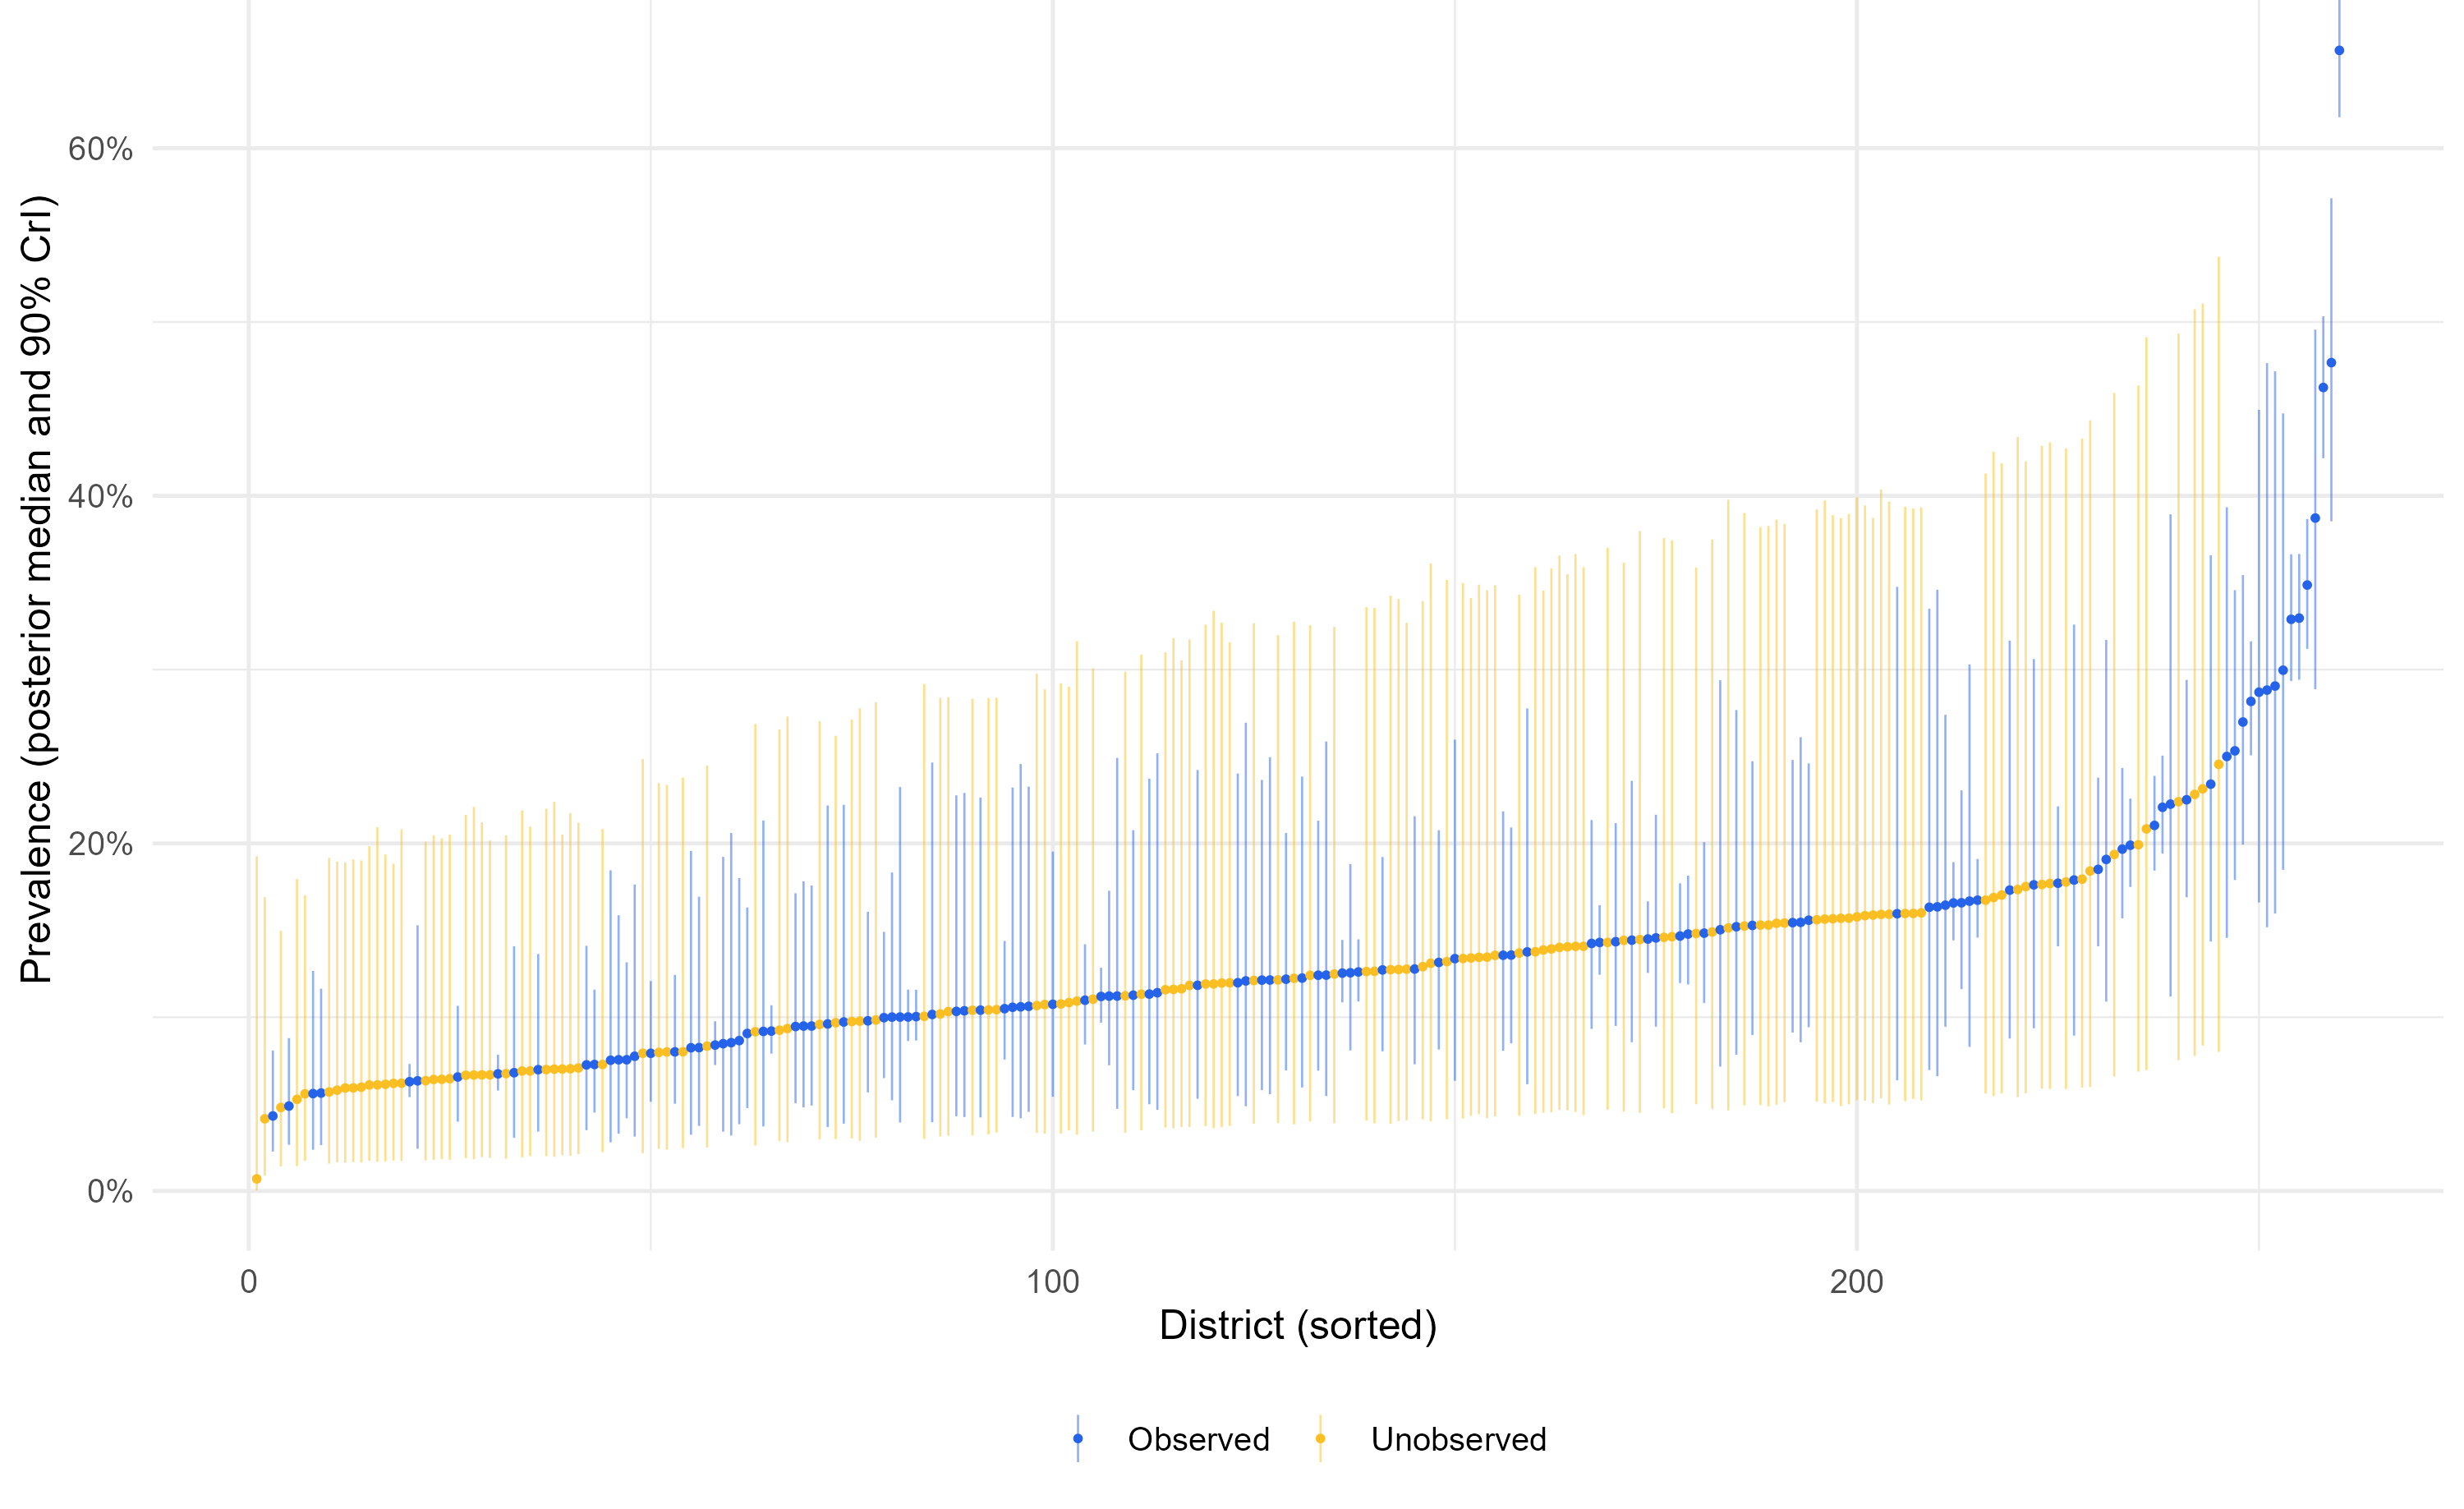
\includegraphics[width=0.7\linewidth,]{caterpillar_plot_ghana_r2} 

}

\caption{District-level prevalence estimates for Ghana 2022 under Model 1 BYM2, sorted by posterior median. Each point is one of the 260 districts with its 90 per cent credible interval. Blue districts contained at least one DHS cluster in 2022 (observed); gold districts contained none (unobserved). Unobserved districts carry visibly wider credible intervals, reflecting their greater reliance on spatial smoothing and the covariate signal\label{fig:caterpillar-gha-r2}}\label{fig:caterpillar-gha-r2}
\end{figure}

\begin{figure}[H]

{\centering 
\includegraphics[width=0.7\linewidth,]{model_comparison_maps_ghana} 

}

\caption{Model 1 estimated under-five malaria prevalence for Ghana 2022: direct estimates (top-left), IID (top-right), ICAR (bottom-left), BYM2 (bottom-right). Districts with no observed clusters are shown in white in the direct panel and filled by the model in the model-based panels. \label{fig:m1-maps}}\label{fig:m1-maps}
\end{figure}

The district-level posterior estimates from this fit are shown in Figure
\textbackslash ref\{fig:caterpillar-gha-r2). The wider credible
intervals on unobserved districts make visible the cost of relying on
spatial smoothing and covariate information rather than direct survey
evidence, and the smooth interleaving of observed and unobserved
districts across the ordered support shows that the model does not
artifactually separate the two groups.

The covariate effects are broadly consistent across the three variants
and credibly identify two of the seven coefficients under the BYM2 fit.
Travel time has a positive effect (\(\beta_5 = 0.21\), \([0.06, 0.35]\))
and log population density a positive effect at the edge of credibility
(\(\beta_6 = 0.34\), with the 90 per cent CrI ranging from \(-0.05\) to
\(0.72\)). Nighttime lights (\(\beta_3\)) and temperature (\(\beta_4\))
have negative point estimates but credible intervals that span zero.
Elevation, rainfall and poverty have credible intervals comfortably
overlapping zero in the BYM2 fit. The implied national paediatric
prevalence from the BYM2 fit is \(14.1\) per cent (\([11.8, 16.5]\)),
consistent with the direct national estimate of \(13.9\) per cent
reported above. The Ghana 2022 fits return a population-prevalence
figure close to the direct estimate without forcing it through the
prior.

\begingroup\fontsize{8}{10}\selectfont

\begin{longtable}[t]{lrrrrr}
\caption{\label{tab:cross-loo}Leave-one-out cross-validation across Ghana Baseline models. ELPD difference is computed against the best model; differences smaller than two standard errors are not statistically distinguishable from zero \citep{vehtari2017}. \label{tab:sens-loo}}\\
\toprule
Model & ELPD diff & SE diff & ELPD & SE(ELPD) & p\_loo\\
\midrule
BYM2 & 0.0 & 0.0 & -106.5 & 7.8 & 7.8\\
IID & -1.6 & 1.6 & -108.0 & 7.7 & 7.7\\
ICAR & -6.4 & 4.1 & -112.8 & 9.3 & 9.3\\
\bottomrule
\end{longtable}
\endgroup{}

The leave-one-out cross-validation comparison across the three variants
is reported in Table 5. The BYM2 variant achieves the best expected log
predictive density at \(-106.5\) (SE \(7.8\)), with the IID variant at
\(\Delta\text{ELPD} = -1.6\) (SE \(1.6\)) and the pure ICAR variant at
\(\Delta\text{ELPD} = -6.4\) (SE \(4.1\)). The pure ICAR variant is the
worst of the three by a margin larger than its standard error: forcing
every district residual through the structured component carries a
measurable predictive cost. The BYM2 and IID variants are within one
standard error of one another in ELPD, so the data alone do not strongly
prefer BYM2 over IID on predictive grounds. We retain BYM2 for the
subsequent models because the BYM2 form contains the IID specification
as the \(\phi = 0\) limit (so choosing it costs nothing in predictive
terms relative to IID), and only the structured component of BYM2 allows
an unobserved district to borrow from its neighbours, which is the
purpose of the framework. The Ghana 2022 baseline therefore establishes
that the BYM2 prior is empirically well-supported at district scale and
is the appropriate working choice for the country-level and
three-country specifications that follow.

\subsection{Model 2: country-level
space-time}\label{model-2-country-level-space-time}

Model 2 was fitted independently to each country with the calendar-year
parameterisation. The fits converged with all rank-normalised
\(\hat{R}\) values at or below 1.027 across the three country fits, and
bulk effective sample sizes in the hundreds to thousands for every
reported parameter. The lowest bulk effective sample size across the
three fits is 155 (for \(\sigma_b\) in the Burkina Faso fit, where the
marginal spatial standard deviation is the largest of the three
countries and the geometry is the most challenging to sample), still
well above the threshold for reliable estimation of posterior medians.
No divergent transitions were reported in any of the three fits.

\begin{table}[!h]
\centering
\caption{\label{tab:spacetime-params}Model 2 (country-level space-time) posterior median estimates with 90\% credible intervals [90\% CrI] for Ghana, Burkina Faso, and Côte d'Ivoire. \label{tab:m2-params-all}}
\centering
\fontsize{8}{10}\selectfont
\begin{tabular}[t]{lccc}
\toprule
Parameter & Ghana (GHA) & Burkina Faso (BFA) & Côte d'Ivoire (CIV)\\
\midrule
\textbf{Space-Time Structure} &  &  & \\
\hspace{1em}~~$\mu$ (Intercept) & -1.11 [-1.21, -1.01] & -0.46 [-0.55, -0.38] & -1.22 [-1.32, -1.11]\\
\hspace{1em}~~$\sigma_b$ (Spatial variance) & 0.16 [0.01, 0.47] & 0.61 [0.13, 1.02] & 0.19 [0.01, 0.61]\\
\hspace{1em}~~$\phi$ (Spatial mixing) & 0.63 [0.26, 0.91] & 0.72 [0.34, 0.93] & 0.64 [0.27, 0.91]\\
\hspace{1em}~~$\sigma_\gamma$ (Temporal variance) & 0.73 [0.66, 0.80] & 0.75 [0.65, 0.84] & 0.68 [0.59, 0.77]\\
\addlinespace
\hspace{1em}~~$\delta$ (Linear time trend) & -0.14 [-0.17, -0.12] & -0.24 [-0.27, -0.22] & 0.09 [0.05, 0.12]\\
\hspace{1em}~~$\delta_{R2-R1}$ (Log-odds shift: R2 vs R1) & -1.15 [-1.33, -0.95] & -2.67 [-2.94, -2.36] & 0.79 [0.47, 1.10]\\
\hspace{1em}~~Odds Ratio (Round 2 vs 1) & 0.32 [0.26, 0.39] & 0.07 [0.05, 0.09] & 2.20 [1.60, 3.01]\\
\textbf{Covariates (Fixed Effects)} &  &  & \\
\hspace{1em}~~$\beta_1$ & -0.10 [-0.20, 0.01] & -0.10 [-0.22, 0.03] & -0.15 [-0.37, 0.08]\\
\addlinespace
\hspace{1em}~~$\beta_2$ & 0.15 [-0.09, 0.39] & 0.05 [-0.12, 0.24] & -0.07 [-0.25, 0.11]\\
\hspace{1em}~~$\beta_3$ & -0.28 [-0.53, -0.02] & -0.12 [-0.19, -0.06] & -0.37 [-0.52, -0.23]\\
\hspace{1em}~~$\beta_4$ & -0.22 [-0.34, -0.10] & 0.07 [-0.18, 0.29] & -0.17 [-0.39, 0.05]\\
\hspace{1em}~~$\beta_5$ & 0.18 [0.08, 0.28] & 0.04 [-0.07, 0.15] & -0.17 [-0.29, -0.06]\\
\hspace{1em}~~$\beta_6$ & 0.13 [-0.13, 0.40] & -0.25 [-0.37, -0.14] & -0.13 [-0.28, 0.03]\\
\addlinespace
\hspace{1em}~~$\beta_7$ & 0.19 [0.03, 0.34] & 0.05 [-0.03, 0.14] & 0.09 [-0.08, 0.26]\\
\textbf{National Prevalence} &  &  & \\
\hspace{1em}~~$p_{national}$ (Round 1) & 0.33 [0.32, 0.35] & 0.70 [0.69, 0.71] & 0.22 [0.21, 0.24]\\
\hspace{1em}~~$p_{national}$ (Round 2) & 0.15 [0.14, 0.16] & 0.19 [0.18, 0.21] & 0.31 [0.30, 0.32]\\
\bottomrule
\end{tabular}
\end{table}

The three countries follow strikingly different trajectories between
rounds. In Ghana, the global intercept is \(\mu = -1.11\)
(\([-1.21, -1.01]\)), the calendar-year slope is \(\delta = -0.143\)
(\([-0.167, -0.119]\)) per year, and the implied between-round logit
shift over the eight-year window between the 2014 and 2022 surveys is
\(\delta_{R2-R1} = -1.15\) (\([-1.33, -0.95]\)), giving a between-round
odds ratio of \(0.32\) (\([0.26, 0.39]\)). The implied national
prevalence falls from \(33.3\) per cent (\([31.7, 34.9]\)) in Round 1 to
\(14.8\) per cent (\([13.5, 16.1]\)) in Round 2. In Burkina Faso, the
global intercept is \(\mu = -0.46\) (\([-0.55, -0.38]\)), the
calendar-year slope is steeper at \(\delta = -0.242\)
(\([-0.268, -0.215]\)) per year, and the implied between-round logit
shift over the eleven-year window between 2010 and 2021 is
\(\delta_{R2-R1} = -2.67\) (\([-2.94, -2.36]\)), giving a between-round
odds ratio of \(0.07\) (\([0.05, 0.09]\)). The implied national
prevalence falls from \(69.6\) per cent (\([68.5, 70.7]\)) in Round 1 to
\(19.3\) per cent (\([17.9, 20.8]\)) in Round 2. Côte d'Ivoire moves in
the opposite direction. The global intercept is \(\mu = -1.22\)
(\([-1.32, -1.11]\)), the calendar-year slope is positive at
\(\delta = +0.087\) (\([0.052, 0.122]\)) per year, and the implied
between-round logit shift over the nine-year window between 2012 and
2021 is \(\delta_{R2-R1} = +0.79\) (\([0.47, 1.10]\)), giving a
between-round odds ratio of \(2.20\) (\([1.60, 3.01]\)). The implied
national prevalence rises from \(22.4\) per cent (\([20.9, 24.1]\)) in
Round 1 to \(31.0\) per cent (\([29.7, 32.4]\)) in Round 2. The contrast
between two countries in rapid retreat and a third moving against the
regional tide is the central empirical finding of this section, and the
sections below show it to be robust to how the data are modelled
jointly.

The spatial parameters tell a complementary story. The marginal spatial
standard deviation \(\sigma_b\) is well identified for Burkina Faso at
\(0.61\) (\([0.13, 1.02]\)), reflecting the country's pronounced
north-to-south transmission gradient. The Ghana and Côte d'Ivoire
estimates are much smaller at \(0.16\) (\([0.01, 0.47]\)) and \(0.19\)
(\([0.01, 0.61]\)) respectively, and their lower 90 per cent bounds
reach close to zero, indicating that after conditioning on covariates
the residual spatial heterogeneity at district scale in these two
countries is modest. The mixing parameter \(\phi\) is close to two
thirds in all three countries, with posterior medians of \(0.63\) in
Ghana, \(0.72\) in Burkina Faso and \(0.64\) in Côte d'Ivoire,
indicating that between a half and roughly three quarters of the
residual spatial variation is geographically structured in each. The
Knorr-Held Type I interaction standard deviation \(\sigma_\gamma\) is
consistent across countries at around \(0.7\) logit units (Ghana
\(0.73\); Burkina Faso \(0.75\); Côte d'Ivoire \(0.68\)). This indicates
a meaningful amount of unstructured district-time variation that
survives conditioning on the spatial, temporal and covariate terms; in
absolute terms it is larger than the marginal spatial standard deviation
in Ghana and Côte d'Ivoire, which says that within those two countries
the district-time-level variation around national trajectories is at
least as large as the time-invariant spatial residual structure.

The covariate effects in Model 2 are country-specific and identify a
pattern of mostly protective effects with some heterogeneity across the
three countries. In Ghana, log population density is positive but the
credible interval narrowly excludes zero in only one direction
(\(\beta_6 = 0.13\), \([-0.13, 0.40]\)); travel time is credibly
positive (\(\beta_5 = 0.18\), \([0.08, 0.28]\)); temperature is credibly
negative (\(\beta_4 = -0.22\), \([-0.34, -0.10]\)); and poverty is
credibly positive (\(\beta_7 = 0.19\), \([0.03, 0.34]\)). In Burkina
Faso, only nighttime lights (\(\beta_3 = -0.12\), \([-0.19, -0.06]\))
and log population density (\(\beta_6 = -0.25\), \([-0.37, -0.14]\))
have credible intervals excluding zero, and both are negative,
consistent with the protective effect of urbanisation. In Côte d'Ivoire,
four covariates have credible intervals excluding zero: nighttime lights
(\(\beta_3 = -0.37\), \([-0.52, -0.23]\)), travel time
(\(\beta_5 = -0.17\), \([-0.29, -0.06]\)), with temperature
(\(\beta_4 = -0.17\), \([-0.39, 0.05]\)) and elevation
(\(\beta_1 = -0.15\), \([-0.37, 0.08]\)) borderline. The
nighttime-lights coefficient is consistently negative across all three
countries (and most credibly so in Côte d'Ivoire), which is the most
stable covariate-prevalence relationship in Model 2 and is a finding the
three-country specifications will sharpen further through partial
pooling.

What the country-level Model 2 cannot do is share information across
borders or pull a regional consensus out of the covariate effects. Côte
d'Ivoire in particular, with the smallest district count, has the widest
credible intervals on the spatial parameters and would benefit most from
borrowing. The three-country models that follow address this, beginning
with the temporally aligned single-time model.

\subsection{Model 3: three-country
single-time}\label{model-3-three-country-single-time-1}

Model 3 fits the second survey rounds of all three countries (Burkina
Faso 2021, Côte d'Ivoire 2021, Ghana 2022) on the combined 724-district
adjacency graph including the 78 cross-border edges. The fit converged
cleanly. The structural parameters from Model 3 establish three things
relevant to what follows. The combined-graph spatial standard deviation
is well identified and the country deviations \(\alpha_c\) order as
expected, with Burkina Faso highest, Côte d'Ivoire intermediate and
Ghana lowest after accounting for the global intercept. The regional
covariate means \(\bar{\beta}_k\) from the hierarchical pooling pick out
nighttime lights as the strongest protective regional effect. The pooled
posterior is consistent with the cross-border specification on
temporally aligned data and serves as the structural baseline for the
two-time Model 4.

\subsection{Model 4: three-country two-time, calendar
year}\label{model-4-three-country-two-time-calendar-year}

Model 4 extends Model 3 to both rounds with country-specific linear
slopes on the centred calendar year. The fit converged with
rank-normalised \(\hat{R}\) values at or below \(1.028\) for all
top-level parameters and bulk effective sample sizes between \(118\)
(the lowest, for \(\alpha_3\), where the country intercept is being
identified jointly with the global mean under the sum-to-zero
constraint) and \(7,452\). The structural and country-specific posterior
summaries are presented in your Model 4 family Table.

The global intercept is \(\mu = -1.14\) (\([-1.33, -0.95]\)) on the
logit scale. The marginal spatial standard deviation is
\(\sigma_b = 0.66\) (\([0.40, 0.91]\)), substantially larger than any of
the country-level \(\sigma_b\) estimates from Model 2, and the mixing
parameter is \(\phi = 0.85\) (\([0.57, 0.96]\)), substantially higher
than any of the country-level \(\phi\) estimates. Two features of this
comparison are worth pulling out. First, the larger \(\sigma_b\)
reflects that, on the combined 724-district graph, the spatial residual
is being asked to absorb not only within-country heterogeneity but also
between-country structure that the country intercepts \(\alpha_c\) do
not fully capture. Second, the high \(\phi\) indicates that the residual
spatial variation is predominantly structured; the shared BYM2 field,
operating across the combined graph with cross-border edges, attributes
more of the residual to the structured component than any of the
country-level fits did. The country deviations are \(\alpha_1 = 0\)
(reference, Ghana), \(\alpha_2 = 0.04\) (\([-0.26, 0.36]\), Côte
d'Ivoire) and \(\alpha_3 = 0.67\) (\([0.36, 0.98]\), Burkina Faso). The
sum-to-zero identification places the country deviations against the
global mean rather than against one another, and Burkina Faso's
\(\alpha_3\) is the most strongly identified, reflecting its much higher
Round 1 prevalence.

The country-specific calendar-year slopes recover the three trajectories
on a per-year scale. Ghana's slope is \(\delta_1 = -0.143\)
(\([-0.166, -0.120]\)) per year, Côte d'Ivoire's is
\(\delta_2 = +0.080\) (\([0.049, 0.110]\)) per year, and Burkina Faso's
is \(\delta_3 = -0.230\) (\([-0.255, -0.206]\)) per year, all tightly
identified. The slopes translate to between-round odds ratios using each
country's actual elapsed years: \(0.32\) (\([0.27, 0.38]\)) for Ghana
(over eight years), \(2.09\) (\([1.56, 2.70]\)) for Côte d'Ivoire (over
nine years), and \(0.08\) (\([0.06, 0.10]\)) for Burkina Faso (over
eleven years). These are within Monte Carlo error of the country-level
Model 2 odds ratios, so the temporal reparameterisation preserves the
between-round comparison exactly while replacing it with a per-year rate
of change directly comparable across countries with different elapsed
windows. The regional mean of the slopes is \(\bar{\delta} = -0.09\)
(\([-0.29, 0.11]\)), with the credible interval spanning zero, and the
between-country slope standard deviation is \(\sigma_\delta = 0.18\)
(\([0.09, 0.43]\)). The regional mean credibly overlapping zero is
informative: the three countries genuinely differ in their direction of
travel rather than sharing a common regional trend, and Model 4 captures
this through \(\sigma_\delta\) rather than collapsing it onto
\(\bar{\delta}\). The implied national prevalences for the three
countries match Model 2 to two decimal places.

The regional covariate means \(\bar{\beta}_k\) identify nighttime lights
as the strongest single protective covariate with
\(\bar{\beta}_3 = -0.19\) (\([-0.43, 0.00]\)), followed by log
population density at \(\bar{\beta}_6 = -0.19\) (\([-0.38, 0.08]\)),
temperature at \(\bar{\beta}_4 = -0.14\) (\([-0.35, 0.10]\)), and
elevation at \(\bar{\beta}_1 = -0.12\) (\([-0.26, 0.04]\)). Rainfall,
travel time and poverty have regional credible intervals that span zero
comfortably. The between-country covariate-slope standard deviations
\(\tau_k\) are between \(0.11\) (for elevation and poverty) and \(0.22\)
(for travel time), indicating that country-specific covariate effects do
not differ enormously around their respective regional means once the
data from the three countries are pooled into the hierarchical
structure. The Knorr-Held Type I interaction standard deviation is
\(\sigma_\gamma = 0.71\) (\([0.66, 0.76]\)), comparable to the
country-level Model 2 values and reflecting that joint estimation has
not concentrated the unstructured space-time variation.

Three substantive features of the Model 4 results stand out. The
country-specific trajectories from Model 2 are preserved and slightly
tightened by the joint fit; the regional covariate pattern identifies
nighttime lights, population density and temperature as the dominant
structural protective factors at the regional scale; and the spatial
residual after conditioning on covariates and country intercepts is
predominantly structured (\(\phi = 0.85\)), consistent with the
substantive expectation that residual variation reflects unmeasured but
spatially smooth determinants such as vector ecology, intervention
history and housing quality.

\subsection{Sensitivity analyses}\label{sensitivity-analyses}

We assess three structural relaxations of Model 4: time-varying
covariate slopes (Model 4a), country-specific BYM2 hyperparameters
(Model 4b), and removal of cross-border edges from the adjacency graph
(edge-deletion). All three are fitted to the same 1,448 district-round
observations, so leave-one-out cross-validation is directly comparable
across them.

\begin{table}[!h]
\centering
\caption{\label{tab:model4all-params}Posterior median estimates with 90\% credible intervals [90\% CrI] across four variants of Model 4. \label{tab:m4-all-variants}}
\centering
\resizebox{\ifdim\width>\linewidth\linewidth\else\width\fi}{!}{
\fontsize{7}{9}\selectfont
\begin{tabular}[t]{lcccc}
\toprule
Parameter & Model 4 (Base) & Model 4a (Time-Varying) & Model 4b (Country BYM2) & Model 4 (Edge Deletion)\\
\midrule
\textbf{Intercept \& Variances} &  &  &  & \\
\hspace{1em}~~$\mu$ (Global Intercept) & -1.14 [-1.33, -0.95] & -1.15 [-1.34, -0.96] & -1.02 [-1.27, -0.42] & -0.68 [-1.32, 0.27]\\
\hspace{1em}~~$\sigma_\gamma$ (Temporal variance) & 0.71 [0.66, 0.76] & 0.70 [0.64, 0.75] & 0.72 [0.67, 0.77] & 0.73 [0.67, 0.78]\\
\hspace{1em}~~$\sigma_\delta$ (Time trend variance) & 0.18 [0.09, 0.43] & 0.18 [0.09, 0.43] & 0.18 [0.09, 0.41] & 0.18 [0.09, 0.44]\\
\textbf{Spatial Parameters} &  &  &  & \\
\addlinespace
\hspace{1em}~~$\sigma_b$ (Global spatial variance) & 0.66 [0.40, 0.91] & 0.71 [0.45, 0.95] & - & 0.50 [0.25, 0.72]\\
\hspace{1em}~~$\sigma_b[1]$ & - & - & 0.13 [0.01, 0.39] & -\\
\hspace{1em}~~$\sigma_b[2]$ & - & - & 0.11 [0.01, 0.40] & -\\
\hspace{1em}~~$\sigma_b[3]$ & - & - & 0.66 [0.41, 0.96] & -\\
\hspace{1em}~~$\phi$ (Global spatial mixing) & 0.85 [0.57, 0.96] & 0.86 [0.63, 0.96] & - & 0.79 [0.46, 0.95]\\
\addlinespace
\hspace{1em}~~$\phi[1]$ & - & - & 0.62 [0.25, 0.90] & -\\
\hspace{1em}~~$\phi[2]$ & - & - & 0.63 [0.26, 0.91] & -\\
\hspace{1em}~~$\phi[3]$ & - & - & 0.72 [0.37, 0.92] & -\\
\textbf{Country Effects ($\alpha$)} &  &  &  & \\
\hspace{1em}~~$\alpha_1$ & 0.00 [0.00, 0.00] & 0.00 [0.00, 0.00] & 0.00 [0.00, 0.00] & 0.00 [0.00, 0.00]\\
\addlinespace
\hspace{1em}~~$\alpha_2$ & 0.04 [-0.26, 0.36] & 0.04 [-0.26, 0.37] & -0.51 [-2.15, 0.95] & -0.24 [-2.55, 1.51]\\
\hspace{1em}~~$\alpha_3$ & 0.67 [0.36, 0.98] & 0.67 [0.34, 1.01] & 0.64 [-0.94, 2.37] & -0.06 [-1.94, 0.82]\\
\textbf{Time Effects ($\delta$)} &  &  &  & \\
\hspace{1em}~~$\bar{\delta}$ (Global time trend) & -0.09 [-0.29, 0.11] & -0.10 [-0.29, 0.11] & -0.10 [-0.29, 0.11] & -0.09 [-0.29, 0.10]\\
\hspace{1em}~~$\delta_1$ & -0.14 [-0.17, -0.12] & -0.14 [-0.16, -0.11] & -0.14 [-0.17, -0.12] & -0.14 [-0.17, -0.12]\\
\addlinespace
\hspace{1em}~~$\delta_2$ & 0.08 [0.05, 0.11] & 0.08 [0.05, 0.10] & 0.08 [0.05, 0.11] & 0.08 [0.05, 0.11]\\
\hspace{1em}~~$\delta_3$ & -0.23 [-0.26, -0.21] & -0.23 [-0.25, -0.21] & -0.23 [-0.26, -0.21] & -0.23 [-0.26, -0.21]\\
\textbf{Covariate Effects ($\bar{\beta}$)} &  &  &  & \\
\hspace{1em}~~$\bar{\beta}_1$ & -0.12 [-0.26, 0.04] & -0.13 [-0.23, -0.02] & -0.12 [-0.25, 0.02] & -0.11 [-0.25, 0.03]\\
\hspace{1em}~~$\bar{\beta}_2$ & -0.01 [-0.20, 0.20] & -0.02 [-0.17, 0.13] & 0.02 [-0.16, 0.22] & 0.00 [-0.19, 0.20]\\
\addlinespace
\hspace{1em}~~$\bar{\beta}_3$ & -0.19 [-0.43, 0.00] & -0.17 [-0.27, -0.08] & -0.21 [-0.46, 0.02] & -0.19 [-0.43, 0.02]\\
\hspace{1em}~~$\bar{\beta}_4$ & -0.14 [-0.35, 0.10] & -0.14 [-0.27, 0.02] & -0.14 [-0.32, 0.12] & -0.12 [-0.35, 0.13]\\
\hspace{1em}~~$\bar{\beta}_5$ & 0.02 [-0.24, 0.26] & 0.01 [-0.10, 0.12] & 0.01 [-0.25, 0.26] & 0.01 [-0.23, 0.24]\\
\hspace{1em}~~$\bar{\beta}_6$ & -0.19 [-0.38, 0.08] & -0.21 [-0.32, -0.07] & -0.17 [-0.38, 0.11] & -0.19 [-0.37, 0.09]\\
\hspace{1em}~~$\bar{\beta}_7$ & 0.08 [-0.05, 0.23] & 0.07 [-0.02, 0.17] & 0.09 [-0.05, 0.24] & 0.09 [-0.06, 0.25]\\
\bottomrule
\end{tabular}}
\end{table}

\subsubsection{Model 4a: time-varying covariate
slopes}\label{model-4a-time-varying-covariate-slopes}

Model 4a allows country-specific covariate slopes to differ between
rounds. The fit converged with rank-normalised \(\hat{R}\) values at or
below \(1.018\) for all top-level parameters and bulk effective sample
sizes between \(141\) and \(6,942\). The structural parameters are
essentially unchanged from Model 4. The global intercept is
\(\mu = -1.15\) (\([-1.34, -0.96]\)), the marginal spatial standard
deviation is \(\sigma_b = 0.71\) (\([0.45, 0.95]\)), the mixing
parameter is \(\phi = 0.86\) (\([0.63, 0.96]\)), and the Knorr-Held Type
I standard deviation is \(\sigma_\gamma = 0.70\) (\([0.64, 0.75]\)). The
country-specific calendar-year slopes are \(\delta_1 = -0.137\)
(\([-0.163, -0.111]\)) for Ghana, \(\delta_2 = +0.076\)
(\([0.047, 0.104]\)) for Côte d'Ivoire, and \(\delta_3 = -0.232\)
(\([-0.254, -0.210]\)) for Burkina Faso, all within Monte Carlo error of
the Model 4 estimates. The regional covariate means \(\bar{\beta}_k\)
are slightly tighter than in Model 4, with nighttime lights at
\(\bar{\beta}_3 = -0.17\) (\([-0.27, -0.08]\)) now credibly excluding
zero, log population density at \(\bar{\beta}_6 = -0.21\)
(\([-0.32, -0.07]\)) credibly negative, and elevation at
\(\bar{\beta}_1 = -0.13\) (\([-0.23, -0.02]\)) also credibly negative.
The between-country covariate-slope standard deviations \(\tau_k\) are
slightly smaller than in Model 4, with most posterior medians between
\(0.05\) and \(0.12\), consistent with the additional Round
2-versus-Round 1 flexibility absorbing some of the heterogeneity that
the time-invariant Model 4 had to channel through \(\tau\). The 42
country-time-specific covariate slopes themselves are largely consistent
between rounds for the same country-covariate pair, with the largest
changes seen in the Ghana temperature and Ghana log population density
slopes; in both cases the Round 2 credible intervals widen and the
between-round change is well within Monte Carlo noise.

\subsubsection{Model 4b: country-specific BYM2
components}\label{model-4b-country-specific-bym2-components}

Model 4b replaces the shared BYM2 hyperparameters with country-specific
ones on the disconnected within-country adjacency graphs. This is the
most challenging fit of the seven for the sampler, and the diagnostics
reflect it. The rank-normalised \(\hat{R}\) for the country deviations
reaches \(1.291\) (\(\alpha_2\)) and \(1.398\) (\(\alpha_3\)), and the
bulk effective sample sizes for these two parameters are \(11\) and
\(9\) respectively, well below the threshold for reliable inference on
their posterior medians. The global intercept \(\mu\) has
\(\hat{R} = 1.145\) and bulk effective sample size 20. These diagnostics
indicate that Model 4b struggles to identify the global intercept and
the country deviations jointly, because removing the cross-border edges
weakens the cross-country anchoring of these parameters and the
sum-to-zero identification on \(\alpha\) then carries a much larger
share of the work. The substantive parameters of interest, on the other
hand, are well sampled: the country-specific calendar-year slopes are
\(\delta_1 = -0.142\) (\([-0.166, -0.120]\)), \(\delta_2 = +0.080\)
(\([0.050, 0.108]\)) and \(\delta_3 = -0.229\) (\([-0.255, -0.205]\)),
all with bulk effective sample sizes in the thousands and \(\hat{R}\) at
or near \(1.00\); and the regional covariate means \(\bar{\beta}_k\) are
similarly well sampled with bulk effective sample sizes between
\(2{,}700\) and \(4{,}300\).

The country-specific spatial standard deviations are
\(\sigma_{b,1} = 0.13\) (\([0.01, 0.39]\)) for Ghana,
\(\sigma_{b,2} = 0.11\) (\([0.01, 0.40]\)) for Côte d'Ivoire, and
\(\sigma_{b,3} = 0.66\) (\([0.41, 0.96]\)) for Burkina Faso. Burkina
Faso's spatial standard deviation is the only one of the three credibly
identified away from zero; the Ghana and Côte d'Ivoire posteriors have 5
per cent lower bounds at \(0.007\) and \(0.008\) respectively,
indicating that almost all of their residual spatial variation in the
combined panel can be explained by the country intercept and covariates
and very little is left for the BYM2 field to absorb. This is consistent
with the country-level Model 2 spatial standard deviations and tells us
that Burkina Faso carries the dominant share of residual spatial
structure in the three-country panel. The country-specific mixing
parameters are \(\phi_1 = 0.62\) (\([0.25, 0.90]\)) for Ghana,
\(\phi_2 = 0.63\) (\([0.26, 0.91]\)) for Côte d'Ivoire and
\(\phi_3 = 0.72\) (\([0.37, 0.92]\)) for Burkina Faso, all above one
half and pointing to predominantly structured residual variation in
every country once the global mean and country intercepts are removed.

\subsubsection{Edge-deletion
sensitivity}\label{edge-deletion-sensitivity}

The edge-deletion specification removes the \(78\) cross-border edges
from the combined graph and refits Model 4 on the resulting disconnected
three-component graph, with the BYM2 hyperparameters held shared across
the three countries and the per-component scaling factor recomputed. As
with Model 4b, the diagnostics show that some of the model-level
identification weakens when cross-border smoothing is removed. The
global intercept \(\mu\) has \(\hat{R} = 1.342\) and bulk effective
sample size \(10\); the country deviations \(\alpha_2\) and \(\alpha_3\)
have \(\hat{R}\) of \(1.506\) and \(1.392\) and bulk effective sample
sizes of \(8\) and \(9\). The substantive parameters of interest are
again well sampled: the country-year slopes have bulk effective sample
sizes in the thousands and \(\hat{R}\) at or near \(1.00\), as do the
regional covariate means.

The substantive estimates from the edge-deletion fit are stable. The
country-year slopes are \(\delta_1 = -0.141\) (\([-0.165, -0.118]\)),
\(\delta_2 = +0.079\) (\([0.049, 0.110]\)) and \(\delta_3 = -0.233\)
(\([-0.256, -0.210]\)), essentially identical to Model 4 within Monte
Carlo noise. The regional covariate effects are within Monte Carlo error
of Model 4, with nighttime lights at \(\bar{\beta}_3 = -0.19\)
(\([-0.43, 0.02]\)) and log population density at
\(\bar{\beta}_6 = -0.19\) (\([-0.37, 0.09]\)). The marginal spatial
standard deviation drops from \(\sigma_b = 0.66\) to \(\sigma_b = 0.50\)
(\([0.25, 0.72]\)), reflecting that some of the spatial variation
previously absorbed by cross-border smoothing is redistributed into the
unstructured Gaussian term, the country intercepts and the now weakly
identified global intercept. The mixing parameter remains high at
\(\phi = 0.79\) (\([0.46, 0.95]\)).

The key inferential point from the edge-deletion sensitivity is that the
substantive parameters of interest, namely the country-year slopes, the
regional covariate effects and the between-country slope variation, are
stable to removing the cross-border edges, while the absolute level
parameters (\(\mu\), \(\alpha_2\), \(\alpha_3\)) become weakly
identified. The cross-border edges in Model 4 are doing identification
work for the level parameters, but the data-driven findings about
trajectories, covariate effects and between-country heterogeneity do not
depend on them. This is a useful negative result: investigators making
slightly different modelling choices about whether to include
cross-border edges would arrive at substantively the same conclusions
about how the three countries' prevalence have moved between rounds and
which covariates carry the dominant regional signal.

\subsubsection{LOO-CV comparison across the cross-border
specifications}\label{loo-cv-comparison-across-the-cross-border-specifications}

Table 6 reports the leave-one-out cross-validation comparison across the
four cross-border specifications. Model 4a achieves the best expected
log predictive density at \(-465.2\) (SE \(21.2\)). Model 4 trails Model
4a by \(3.4\) ELPD units against a standard error of the difference of
\(4.9\) (\(0.7\) standard errors), the edge-deletion specification
trails by \(2.3\) units against \(4.9\) (\(0.5\) standard errors), and
Model 4b trails by \(5.9\) units against \(5.3\) (\(1.1\) standard
errors). All four specifications are within roughly six ELPD units of
one another against standard errors of around five, and none of the
three structural relaxations of Model 4 produces a detectable
improvement in expected predictive performance. The pareto-smoothed
importance sampling estimates of effective parameters (\(p_\text{loo}\))
cluster around \(591\) to \(595\) for the four fits, reflecting that all
four operate at comparable model complexity in the LOO sense.

\begingroup\fontsize{8}{10}\selectfont

\begin{longtable}[t]{lrrrrr}
\caption{\label{tab:sens-loo}Leave-one-out cross-validation across the cross-border two-time models. ELPD difference is computed against the best model; differences smaller than two standard errors are not statistically distinguishable from zero \citep{vehtari2017}. \label{tab:sens-loo}}\\
\toprule
Model & ELPD diff & SE diff & ELPD & SE(ELPD) & p\_loo\\
\midrule
Model 4a (time-varying betas) & 0.0 & 0.0 & -465.2 & 21.2 & 591.2\\
Edge-deletion (within-country only) & -2.3 & 4.9 & -467.5 & 21.3 & 593.1\\
Model 4 (shared BYM2, full graph) & -3.4 & 4.9 & -468.6 & 21.1 & 594.3\\
Model 4b (country-specific BYM2) & -5.9 & 5.3 & -471.2 & 21.5 & 594.9\\
\bottomrule
\end{longtable}
\endgroup{}

Model 4 is therefore retained as the working three-country two-time
specification on parsimony grounds. Model 4a is preferred by point ELPD,
but the difference is well within one standard error and Model 4 with
its time-invariant covariate slopes is the simpler model. Model 4b is
preferred by neither parsimony nor ELPD; while it identifies Burkina
Faso's distinctive spatial structure, it does so at the cost of much
weakened identification of the country intercepts. The edge-deletion
specification offers neither a predictive nor a parsimony advantage and
weakens identification of the level parameters substantially.

\subsubsection{Convergence and Mixing}\label{convergence-and-mixing}

Convergence diagnostics for all fits followed the rank-normalised
\(\widehat{R}\) statistic and bulk and tail effective sample sizes
\citep{vehtari2021}, with numerical values reported alongside each model
summary above. Figures \ref{fig:trace-plots} and \ref{fig:rank-plots}
show representative visual checks: trace plots for the Model 1 Ghana
2022 BYM2 cross-section, and rank histograms for the Model 4
three-country two-time fit. The chains overlap freely with no visible
trend or stickiness, and the rank histograms are approximately level
with no chain-specific dominance. The same diagnostic battery was
applied to every fit and passed on the substantive parameters of
interest, with the only exceptions being the global intercept and
country deviations under Model 4b and the edge-deletion specification,
which were flagged explicitly in their subsections.

\begin{figure}[H]

{\centering 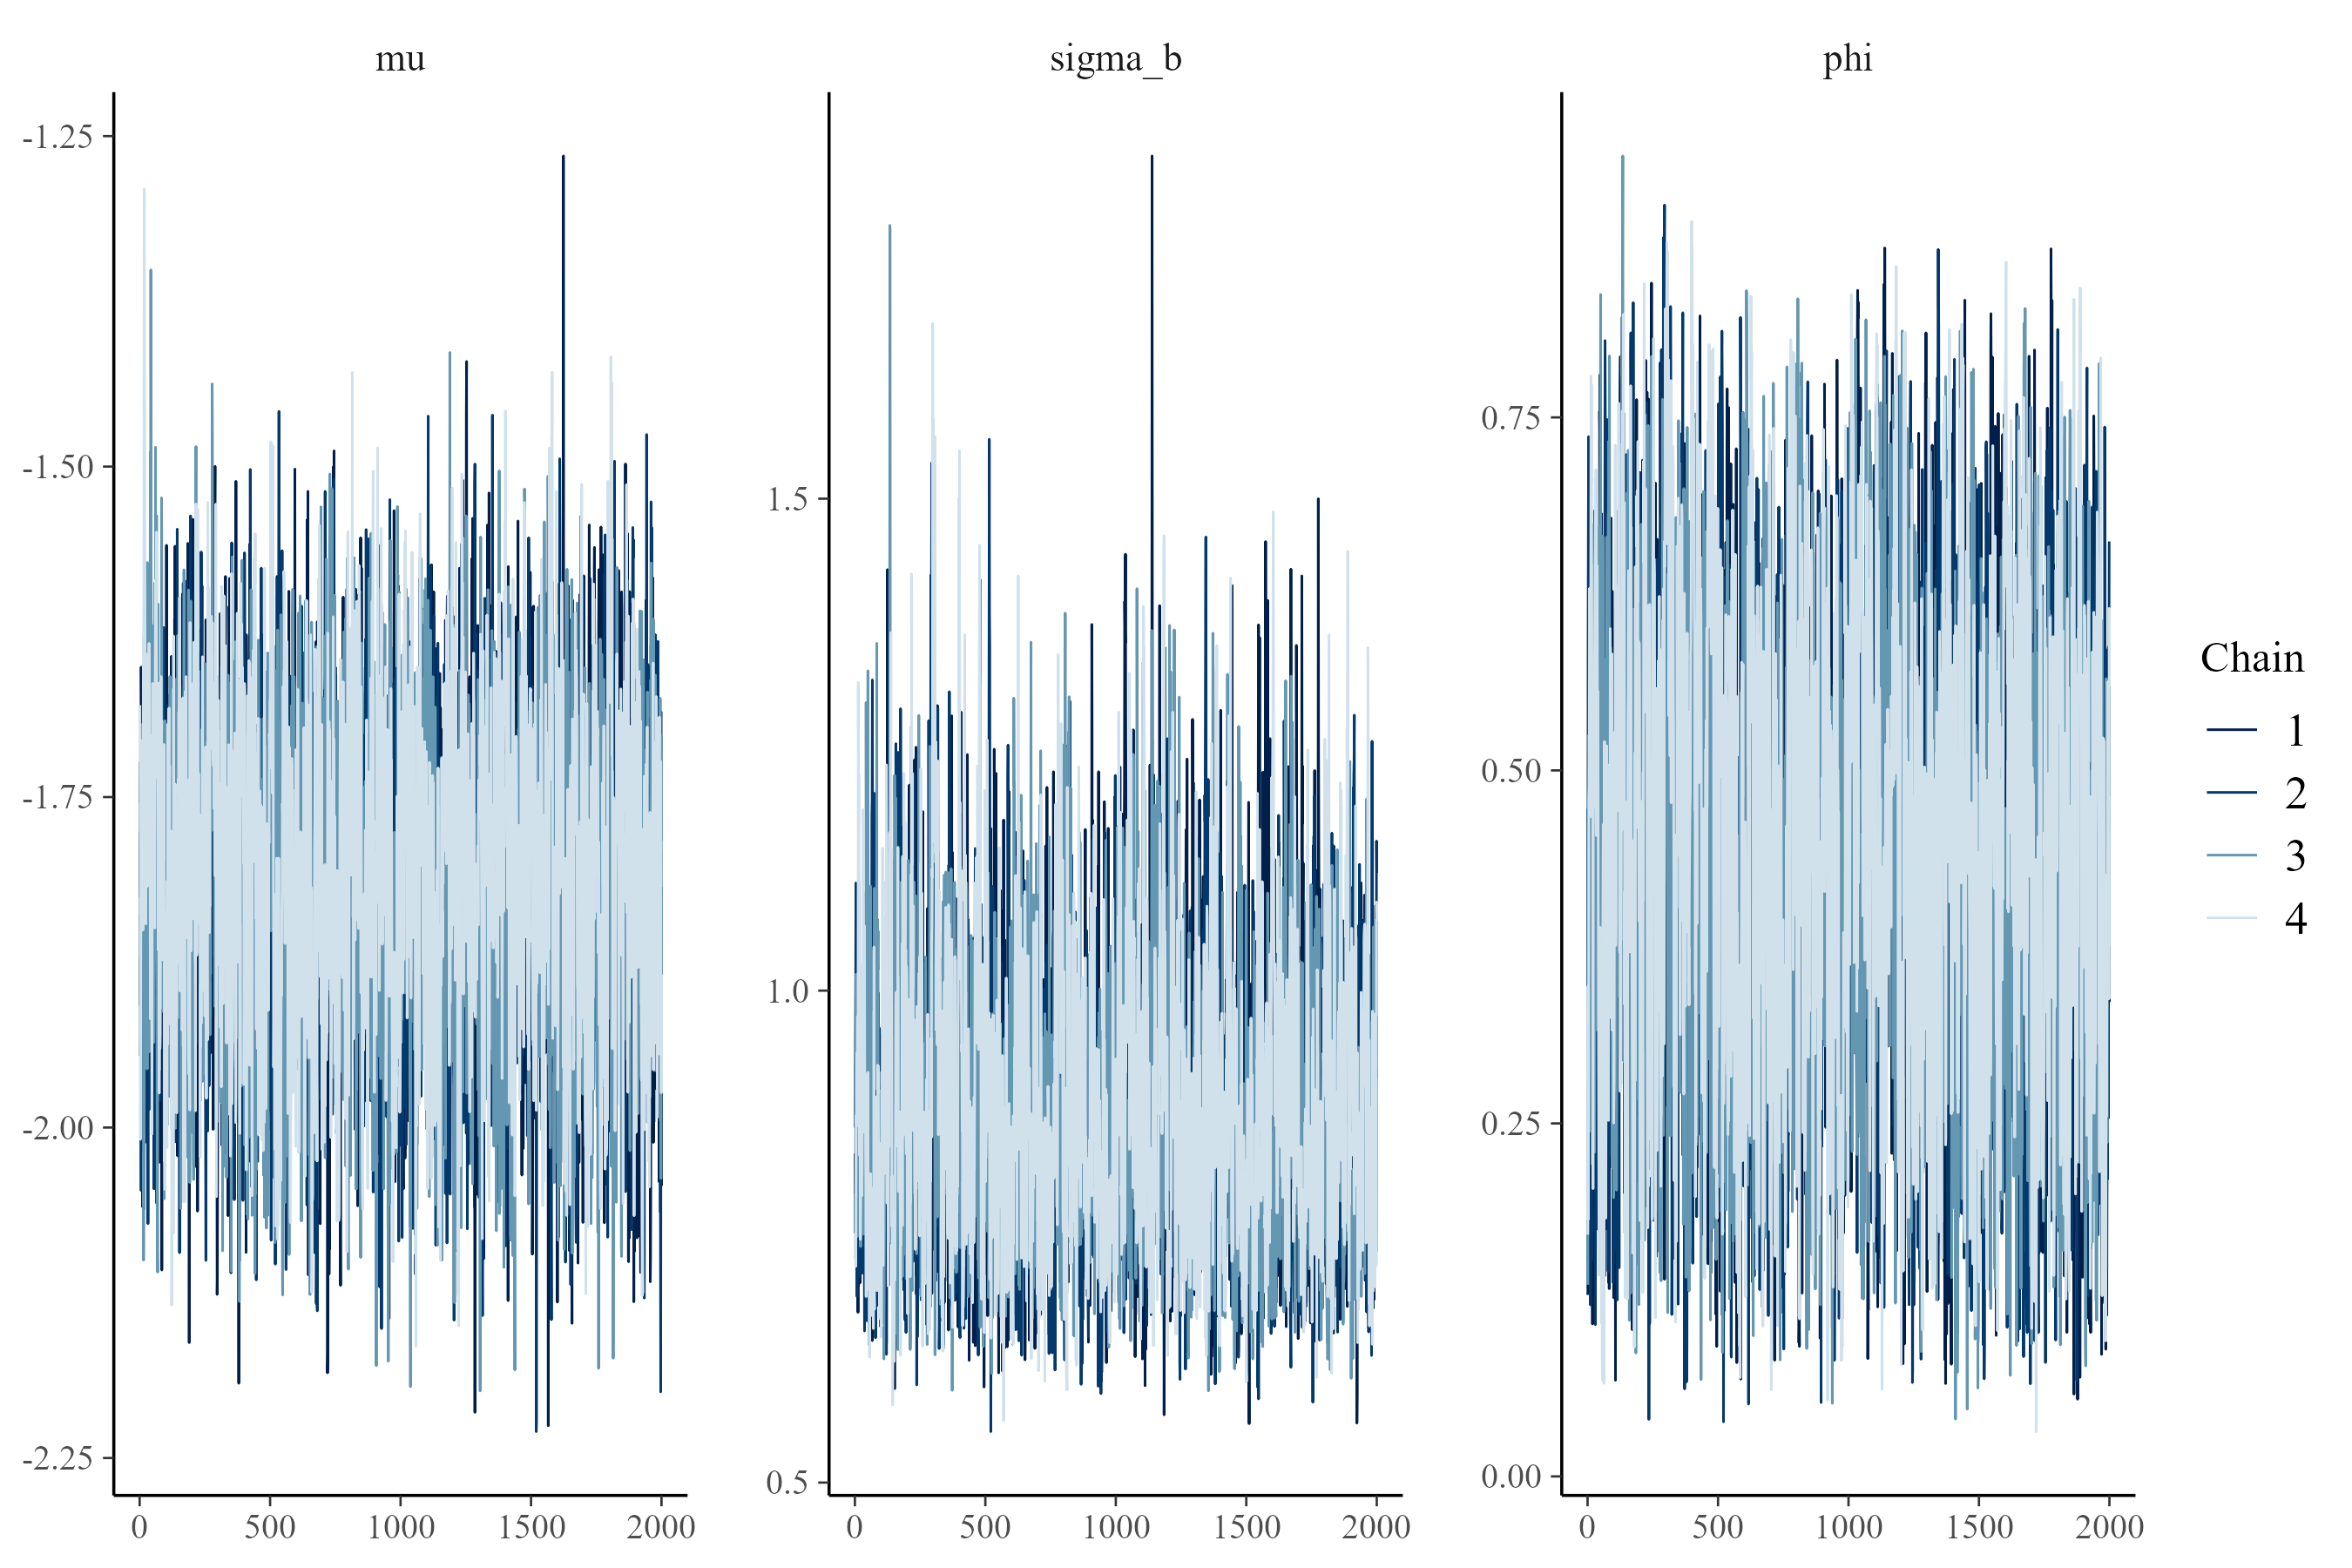
\includegraphics[width=0.7\linewidth,]{trace_plots} 

}

\caption{Trace plots from the Model 1 Ghana 2022 BYM2 fit. Four parallel HMC chains, 2000 post-warmup iterations each.\label{fig:trace-plots}}\label{fig:trace_plots}
\end{figure}

\begin{figure}[H]

{\centering 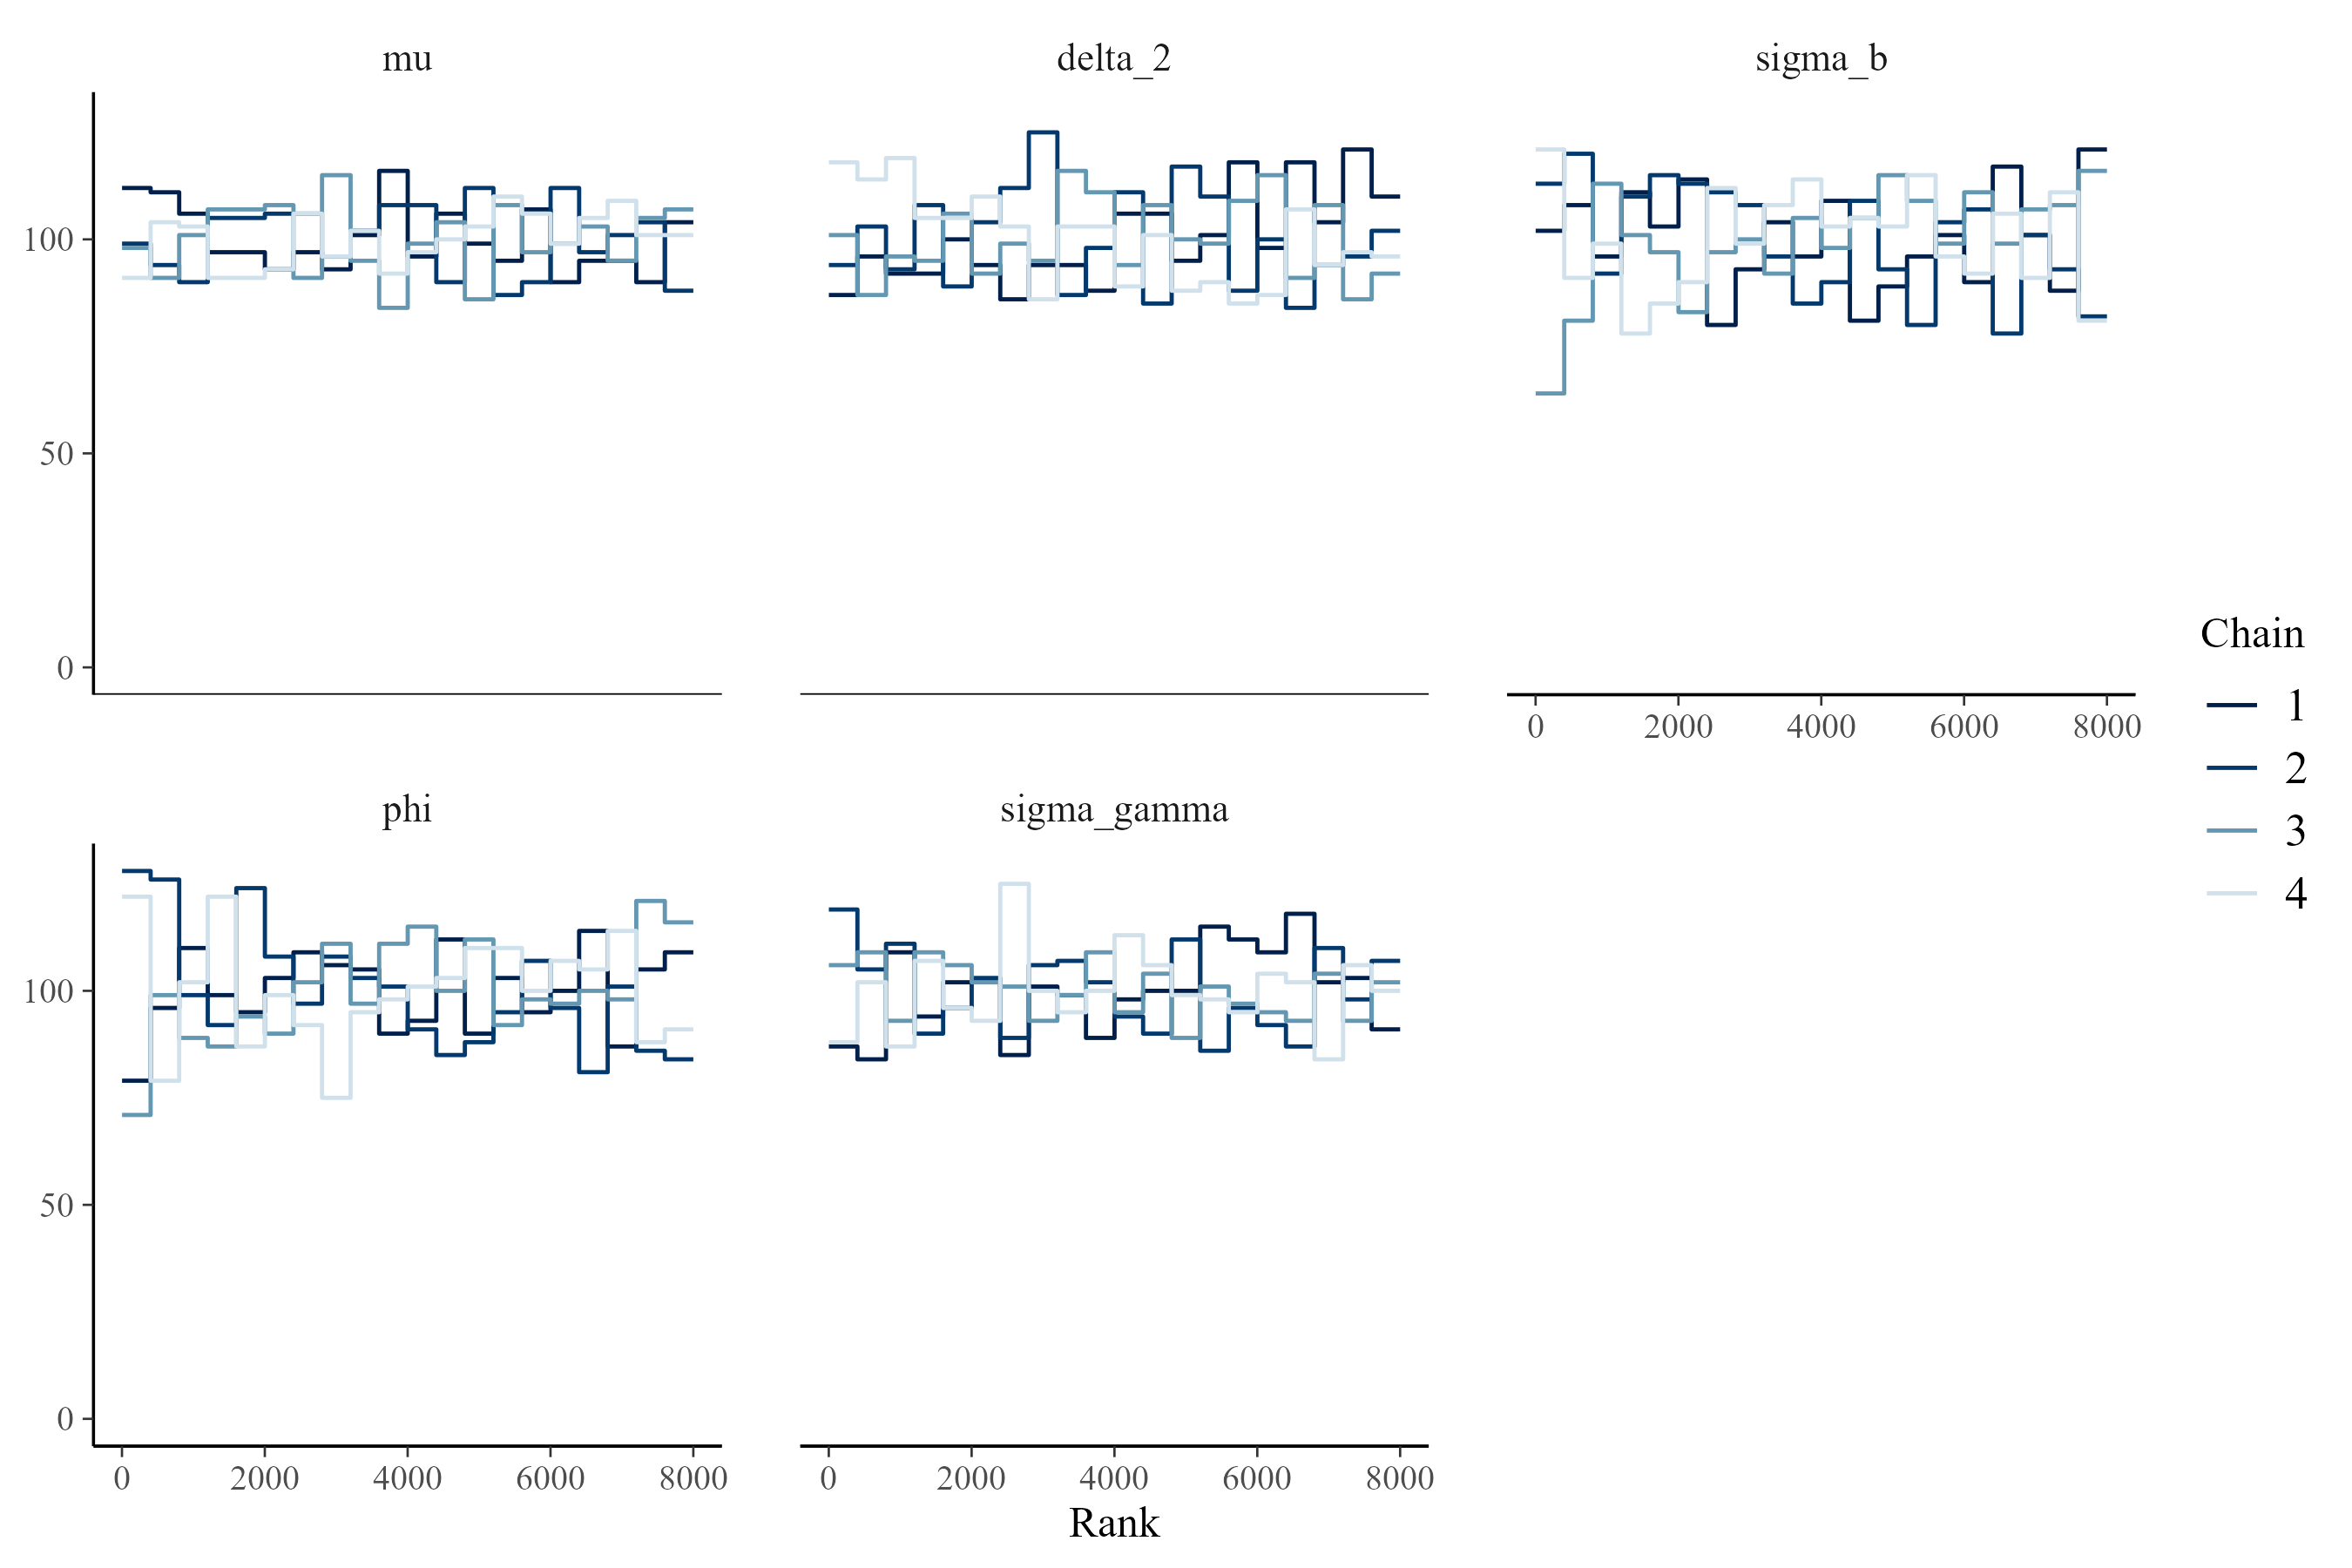
\includegraphics[width=0.7\linewidth,]{rank_plots} 

}

\caption{Rank histograms for the structural parameters of the Model 4 three-country two-time fit. Approximately level bins across the rank space and absence of chain-specific dominance indicate well-mixing chains.\label{fig:rank-plots}}\label{fig:rank_plots}
\end{figure}

\begin{figure}[H]

{\centering 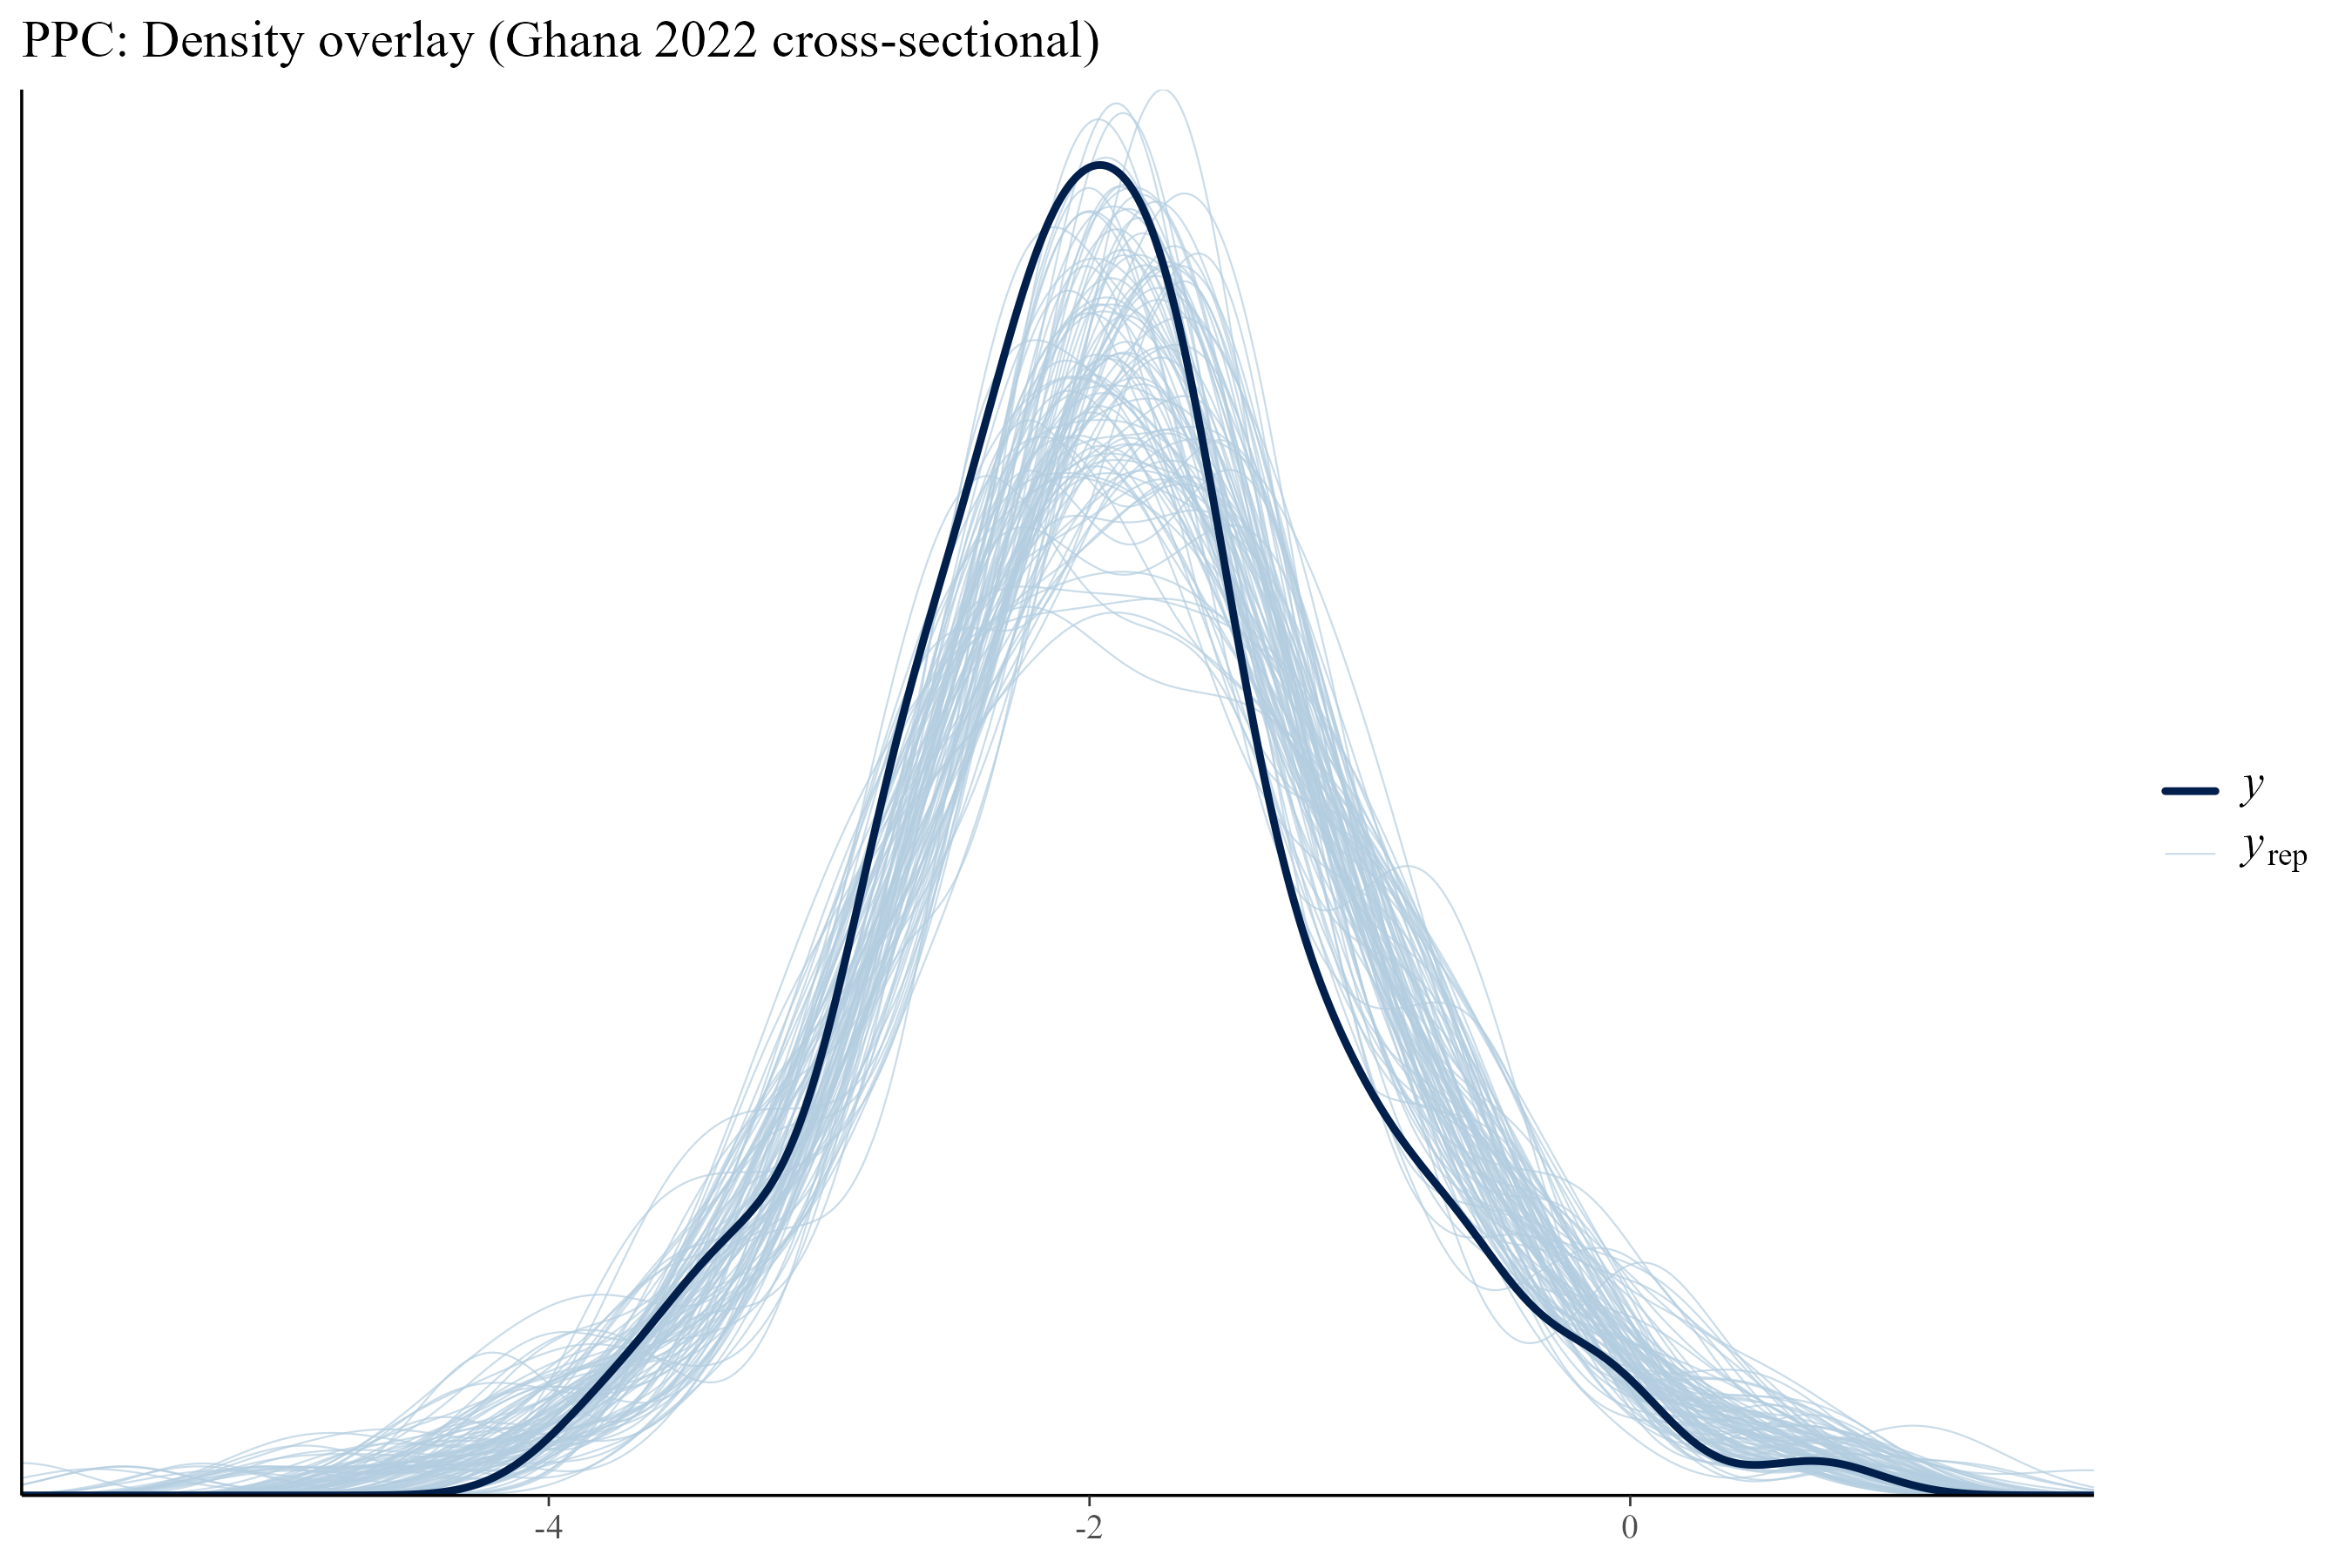
\includegraphics[width=0.7\linewidth,]{ppc_density} 

}

\caption{Posterior predictive density overlay for the Ghana 2022 cross-sectional fit. The solid dark line is the observed density of the direct logit-prevalence estimates; the light traces are the densities of the corresponding posterior predictive replicates. The observed density lies inside the predictive envelope, with a slight under-prediction in the right tail.\label{fig:ppc-density}}\label{fig:ppc-density}
\end{figure}

\begin{figure}[H]

{\centering 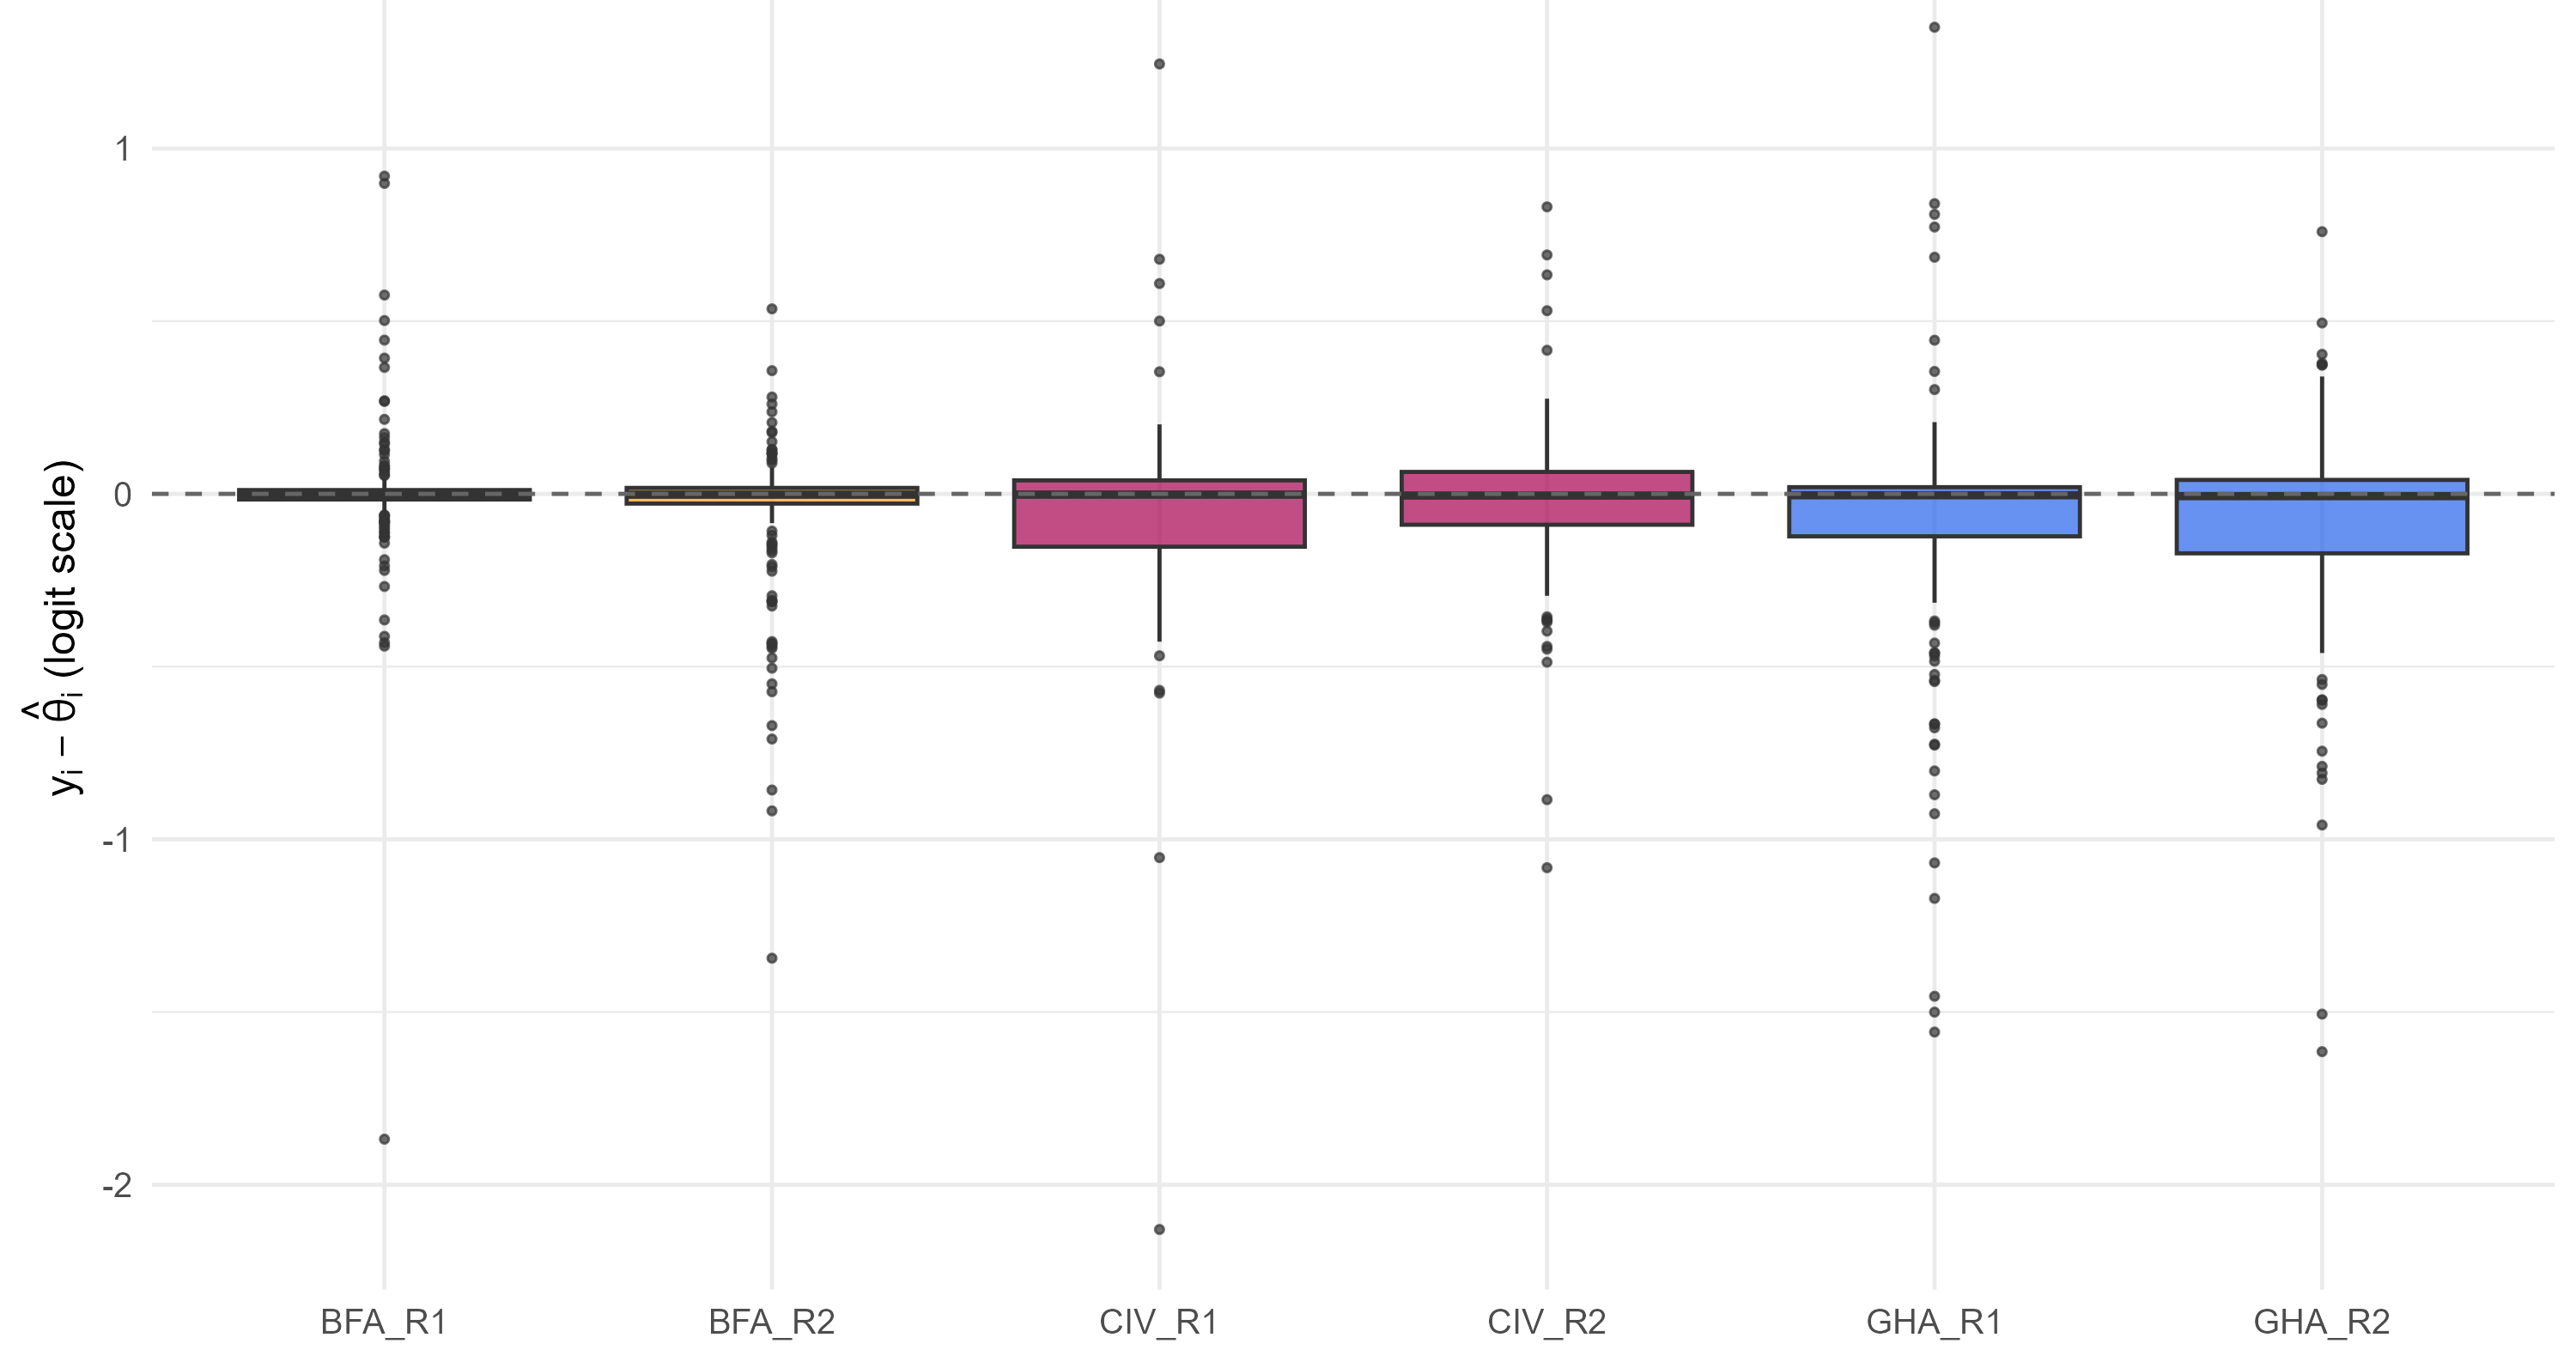
\includegraphics[width=0.7\linewidth,]{residual_boxplot_country_time} 

}

\caption{Raw residuals on the logit scale by country and round under the three-country two-time Model 4 fit. Boxes are approximately centred on zero across all six country-rounds; the slight negative median in the Côte d'Ivoire and Ghana panels is consistent with mild under-prediction at the upper end of the prevalence range.\label{fig:residual-boxplot-country-time}}\label{fig:residual-boxplot}
\end{figure}

Posterior predictive checks support the adequacy of the model fit. The
density overlay for the Ghana 2022 cross-sectional fit Figure
\ref{fig:ppc-density} shows the observed density of the direct
logit-prevalence estimates lying inside the envelope of posterior
predictive replicates, with a slight under-prediction visible in the
right tail of the distribution. Raw residuals by country-round under the
three-country Model 4 fit Figure \ref{fig:residual-boxplot-country-time}
are approximately centred on zero across all six country-rounds, with a
slight negative median in the Côte d'Ivoire and Ghana panels indicating
mild under-prediction at the upper end of the prevalence range. Neither
pattern materially affects the substantive parameter posteriors.

\section{Discussion}\label{discussion}

\label{sec:discussion}

This study presents a three-country area-level Bayesian small area
estimation of under-five malaria prevalence at admin-2 district scale
across Burkina Faso, Côte d'Ivoire and Ghana, combining successive DHS
rounds with environmental and social covariates. The Bayesian
Fay-Herriot framework with BYM2 spatial prior recovered three sharply
divergent country trajectories that are consistent across the
country-level and three-country specifications and through three
structural sensitivity analyses: substantial decline in Burkina Faso and
Ghana between rounds, and an increase in Côte d'Ivoire. At the regional
level the model identifies a small set of environmental and demographic
covariates with credibly protective effects and locates the residual
spatial variation predominantly in the structured component of the BYM2
field. The contribution of this work is the joint application of
established components of the area-level small area estimation tradition
\citep{wu2021} to under-five malaria prevalence across three West
African countries on a shared adjacency graph that respects ecological
rather than administrative boundaries, with country-specific
calendar-year slopes hierarchically pooled around a regional mean and a
formal sensitivity battery around the cross-border specification.
Comparable prior work has applied small area estimation to malaria at
communal level in Burkina Faso \citep{bassinga2024} and to
spatio-temporal malaria risk in Rwanda using survey and routine data
\citep{semakula2023}, and multi-country small area estimation has been
applied to HIV across East and Southern Africa using a shared adjacency
graph \citep{saldarriaga2020}; the framework presented here brings these
elements together at admin-2 district scale across three contiguous West
African countries.

The Burkina Faso decline, with posterior median prevalence falling from
roughly 70\% in 2010 to below 20\% in 2021, aligns temporally with the
country's seasonal malaria chemoprevention programme, launched in 2014
and scaled rapidly thereafter. Multiple independent evaluations have
documented substantial SMC-attributable reductions in paediatric malaria
under routine programme conditions: a quasi-experimental study in Kaya
District estimated protective effects of 51\% on point prevalence and
62\% on period prevalence in 2014-2015 \citep{druetz2018};
national-scale assessments confirmed the effect across SMC and non-SMC
health districts \citep{kirakoya2022}; and a DHS-based analysis of the
2010, 2014 and 2017 surveys detected reduced odds of RDT-positive
malaria for up to two months post-SMC \citep{cola2022}. The Ghana
decline between 2014 and 2022, while more moderate, is consistent with
the broader West African trend documented by Malaria Atlas Project
geostatistical mapping \citep{bhatt2015, weiss2020} and with the
trajectory targeted by the country's model-supported malaria programme
\citep{awine2017}; the most recent World Malaria Report places Ghana
among the countries showing measurable progress towards the 2030
burden-reduction targets \citep{who2024}. The Côte d'Ivoire trajectory
cuts against this regional pattern. Our model places paediatric
prevalence rising from approximately 22\% in 2012 to 31\% in 2021, in
agreement with the official 2021 DHS report which records a national
increase from 18\% in 2011 to 26\% \citep{civdhs2021}, and with a recent
multi-country geospatial analysis that identifies Côte d'Ivoire as one
of the consistently high-prevalence countries in the region
\citep{aide2025}. Two structural factors plausibly contribute. First,
seasonal malaria chemoprevention has not been deployed nationally in
Côte d'Ivoire over the study window; the country's first SMC pilot was
only initiated in 2021 in the Dikodougou health district
\citep{kangah2024}, in stark contrast to Burkina Faso's national
rollout. Second, the dominant vector \emph{Anopheles gambiae sensu lato}
across coastal Côte d'Ivoire showed strong pyrethroid resistance in
bioassays conducted between 2018 and 2020, with mortality remaining
below 98\% even at ten-fold the standard diagnostic dose
\citep{yokoly2024}. Our framework cannot causally attribute any of the
trajectories to specific programmatic decisions, but the contrast
between Burkina Faso's national SMC programme and Côte d'Ivoire's
absence of one is the most striking structural difference relevant to
their divergent paths.

An informal external comparison with the Malaria Atlas Project surfaces,
which estimate annual \emph{Plasmodium falciparum} parasite rate in
children aged 2-10 (PfPR\(_{2-10}\)) using a unit-level Gaussian
geostatistical framework drawing on a broader data ecosystem than the
DHS alone, supports the direction of two of the three country
trajectories recovered here and identifies the Côte d'Ivoire trajectory
as the point of divergence between the two approaches. For Burkina Faso,
MAP's national PfPR\(_{2-10}\) falls from approximately 73 \% in 2010 to
26 \% in 2021, in close agreement with our 70 \% to 19 \% decline in DHS
RDT-positive U5 prevalence; the magnitude of the absolute level in 2010
is also strikingly similar across the two methods despite the metric and
age-band differences. For Ghana, MAP shows a similar decline from
approximately 46 \% in 2014 to 17 \% in 2022, again in directional
agreement with our 33 \% to 15 \% decline. For Côte d'Ivoire, MAP's
surface shows a decline from approximately 48 \% in 2012 to 35 \% in
2021, which is in the opposite direction from the rise recovered by our
model and confirmed by the 2021 DHS report \citep{civdhs2021}. The two
methodological traditions are not directly substitutable: our model uses
only DHS RDT records and operates at admin-2 with a discrete adjacency
graph, whereas the MAP surface unifies multiple data ecosystems
including routine surveillance into a continuous geostatistical field,
and the discrepancy likely reflects the different ways the two methods
weight DHS evidence against routine case data and against historical
baselines. Both methods agree that Côte d'Ivoire remains a
moderate-to-high-prevalence country and a regional outlier within the
West African declining trend; they disagree on whether the
within-country trajectory between 2012 and 2021 is upward or downward,
which is itself an informative finding and is a question that a formal
MAP-versus-SAE concordance analysis at district scale would be well
positioned to resolve.

A consistent feature across all the country-level and three-country
specifications is that the residual spatial variation, after
conditioning on covariates and the temporal component, is predominantly
structured rather than unstructured. The BYM2 mixing parameter
\(\varphi\), which represents the proportion of the marginal spatial
variance attributable to the geographically smooth ICAR component, has
posterior medians of approximately 0.6 to 0.7 across the country-level
Model 2 fits and rises to 0.85 in the three-country Model 4
specification. This pattern indicates that between roughly half and over
four-fifths of the unexplained spatial variation is shared between
neighbouring districts rather than being district-specific noise.
Substantively this is consistent with the prevailing view that the
unmeasured determinants of \emph{Plasmodium falciparum} transmission are
themselves spatially smooth processes that operate at scales larger than
a single district. These determinants include vector species composition
and abundance, breeding-site availability tied to land use and surface
water management practices such as small dams, irrigation schemes and
seasonal water bodies, housing quality, intervention coverage history
and the geographic accessibility of clinical services. The absence of
land use, surface water management and intervention coverage covariates
from our covariate set is a recognised limitation that we return to in
the limitations subsection, and it is itself a structural reason the
BYM2 field absorbs as much of the residual spatial variation as it does.
The continental geostatistical surfaces of the Malaria Atlas Project
show pronounced and coherent spatial structure in West Africa over
successive years \citep{bhatt2015, weiss2020}, and recent district and
communal level SAE in Burkina Faso has similarly emphasised
heterogeneous but spatially clustered prevalence with rural communes
carrying disproportionately higher risk \citep{bassinga2024}. A
geospatial analysis of DHS data across eight West African countries also
reports marked spatial heterogeneity in paediatric malaria prevalence
with hotspots concentrated in Benin and Côte d'Ivoire and lower
prevalence in Ghana \citep{aide2025}. The high posterior \(\varphi\)
recovered specifically by our three-country Model 4 reflects an
additional feature of the shared adjacency graph: the BYM2 field absorbs
both within-country residual structure and between-country structure
that the country intercepts \(\alpha_c\) do not fully capture, which is
consistent with the cross-border nature of transmission processes that
respect ecology rather than administrative boundaries
\citep{riebler2016}.

Among the seven covariates included in the model, the strongest and most
consistent protective signal at the regional level comes from nighttime
lights, which has a credibly negative posterior under Model 4a and
consistent negative point estimates across the country-level Model 2
fits, with Burkina Faso and Côte d'Ivoire showing credible exclusion of
zero. Log population density follows the same pattern, with a regional
mean of approximately \(-0.21\) under Model 4a credibly excluding zero,
and elevation joins these two covariates as credibly negative in the
time-varying specification. These three covariates together describe the
urbanisation gradient across the three countries: densely populated,
electrified, lower-relief districts are associated with reduced
under-five malaria prevalence at the regional scale. This finding is
consistent with the broader urban-malaria literature, which has
documented lower transmission intensity in urban environments owing to
better housing quality, improved drainage and water management that
suppresses vector breeding sites, higher access to clinical services and
treatment, and reduced human-vector contact relative to rural settings
\citep{bhatt2015, weiss2020}. The recent multi-country geospatial
analysis of West African DHS data identifies similar associations, with
urban residence and improved housing emerging as protective factors
across the eight countries analysed \citep{aide2025}, and the
communal-level SAE in Burkina Faso likewise emphasises substantially
higher asymptomatic carriage in rural communes than in urban ones
\citep{bassinga2024}. Temperature shows a consistently negative point
estimate at the regional level with credible intervals that narrowly
span zero in the time-invariant Model 4 specification; the negative
direction is consistent with above-optimal mean temperatures suppressing
vector survival in some districts, although the signal is too uncertain
at our resolution to be interpreted strongly. The remaining covariates,
rainfall, travel time and multidimensional poverty, do not credibly
differ from zero at the regional mean. The between-country slope
standard deviations \(\tau_k\) range between approximately 0.11 and
0.22, indicating that the country-specific slopes do not depart strongly
from the regional means once the data from the three countries are
jointly modelled, although the country-level Model 2 fits identify a
small number of country-specific effects worth noting: Ghana shows a
credibly positive coefficient on multidimensional poverty in keeping
with the expected positive association between poverty and malaria
burden, while Côte d'Ivoire shows a credibly negative coefficient on
travel time consistent with more accessible districts showing lower
transmission intensity.

\subsection{Limitations and weaknesses}\label{sec:limitations}

Several limitations apply to this analysis and should temper the
interpretation of the findings.

\textbf{Data resolution and measurement.} Access to clean district-level
census data for the social covariates was possible only for Ghana, where
the Ghana Statistical Service publishes admin-2 poverty and education
figures from the 2010 and 2021 censuses. For Burkina Faso and Côte
d'Ivoire no equivalent admin-2 census source was available within the
timeframe of the project, and the social covariate used in the
multi-country specifications is the subnational Multidimensional Poverty
Index published on the Humanitarian Data Exchange by the Oxford Poverty
and Human Development Initiative. This index is published at the
regional (admin-1) level for both countries, so every district within a
region carries the same value, and within-region variation in poverty is
absorbed into the spatial random effect rather than into the poverty
coefficient. It is also itself a derived indicator computed from DHS and
MICS surveys rather than a census measurement, so the covariate carries
its own modelling uncertainty that the Fay-Herriot framework treats as
if it were observed without error. The DHS RDT outcome is based on
detection of the \emph{Plasmodium falciparum} HRP2 antigen, and
\emph{pfhrp2/3} gene deletions have been documented in West Africa with
rising prevalence; what we estimate is RDT-positive prevalence, which
may diverge from true infection prevalence where these deletions are
common.

\textbf{Modelling assumptions.} The sampling variance \(\psi_{it}^2\) is
treated as known and fixed at its design-based estimate, following the
standard Fay-Herriot convention \citep{fay1979, you2002}. For districts
with very few clusters this design-based estimate is itself uncertain,
and the framework does not propagate that uncertainty. The BYM2 spatial
field is also assumed time-invariant in Models 3, 4, 4a and 4b. The
dominant ecological drivers of the regional gradient move on decadal
timescales and a single field is substantively defensible, but with only
two rounds the data cannot strongly test the assumption, and Knorr-Held
Type II and higher interactions that would let the spatial structure
evolve are not separately identified \citep{knorrheld2000, goicoa2018}.

\textbf{Missing intervention and environmental covariates.} The
covariate set captures structural and environmental determinants of
transmission at the resolution at which open-access remote-sensing
products and HDX-hosted social indicators are available, but does not
include intervention coverage or several environmental layers known to
drive vector ecology. Insecticide-treated net distribution, indoor
residual spraying, intermittent preventive treatment in pregnancy and
seasonal malaria chemoprevention are spatially and temporally
heterogeneous across the three countries, so their omission means the
model describes the between-round trajectories without being able to
attribute them to specific intervention rollouts. This is most
consequential for Burkina Faso, where the rollout of seasonal malaria
chemoprevention in the Sahel from 2014 onwards is the most likely
proximate driver of the steep decline observed between 2010 and 2021,
and for Côte d'Ivoire, where the absence of a national SMC programme
over the study window is the most likely structural reason the country's
trajectory diverges from its neighbours. The most coherent
district-level source of intervention coverage for all three countries
is the DHS household roster itself, which is subject to the same patchy
district coverage the framework was set up to address, so a coherent
extension would need to smooth intervention coverage through an SAE step
of its own before plugging it in. The covariate set also omits several
environmental layers that are known to mediate vector breeding-site
availability and human-vector contact: district-level land use and land
cover (including agricultural intensity, urban footprint and forest
cover), surface water management infrastructure (small dams, irrigation
schemes and seasonal water bodies), and housing-quality proxies (roof
and wall material, electricity access). These omissions are themselves a
structural reason the BYM2 spatial field absorbs as much of the residual
spatial variation as it does.

\textbf{External validation.} No independent district-level
gold-standard malaria prevalence dataset is available for the three
study countries. The Malaria Atlas Project provides continuous
geostatistical surfaces from a partially overlapping data ecosystem and
is a useful regional reference, but it uses a different modelling
tradition and is itself a modelled product; the informal national-level
comparison reported above shows directional agreement for Burkina Faso
and Ghana and a methodologically informative discrepancy for Côte
d'Ivoire. A formal MAP-versus-SAE concordance analysis at district scale
would be informative for both modelling traditions and is set out as a
natural next step.

\subsection{Future Work}\label{future-work}

The most immediate extension is to add further West African countries to
the shared adjacency graph, with the Togo 2013 and forthcoming 2026 DHS
rounds as the natural next test cases. Upcoming national censuses in the
Democratic Republic of the Congo, Nigeria, Cameroon and Sierra Leone
would unlock admin-2 social covariates directly from census, addressing
the regional-resolution limitation that affects Burkina Faso and Côte
d'Ivoire in the present work. The most consequential substantive
extension is the incorporation of district-level intervention coverage
(insecticide-treated nets, IPTp, seasonal malaria chemoprevention) as
time-varying covariates, smoothed through a coupled SAE step on the DHS
household roster, which would let the framework attribute observed
trajectories to specific intervention rollouts rather than only to
environmental and demographic correlates.

\section{Conclusion}\label{conclusion}

\label{sec:conclusion}

This study documents three sharply divergent country trajectories in
under-five malaria prevalence across Burkina Faso, Côte d'Ivoire and
Ghana at admin-2 district resolution. The Bayesian Fay-Herriot framework
with BYM2 spatial prior on a shared cross-border adjacency graph
recovers country-specific transmission dynamics within a single coherent
statistical framework and produces district-level posterior estimates
with the full uncertainty propagation appropriate for sub-national
programme planning. The trajectories are robust across country-level and
three-country specifications and through three structural sensitivity
analyses, and they are corroborated for Burkina Faso and Ghana by
independent national-level estimates from the Malaria Atlas Project.
Regional aggregates obscure these country-specific dynamics: three
contiguous West African countries moved in opposite directions on
under-five malaria prevalence over the same decade. Country-specific
reporting at district scale, with full posterior uncertainty, is the
resolution at which sub-national malaria programme decisions are
actually made.

\section{Code and Data Availability}\label{code-and-data-availability}

The full analysis code is publicly available at
\url{https://github.com/SAHagen/HDS5106}. The repository contains the
methodological workbook
(\texttt{small\_area\_estimation\_project\_final.Rmd}), the standardised
covariate panels for the seven district-level covariates committed as
CSV files, and the supporting helper scripts. The processed and
standardised covariates being included as CSVs means the upstream
covariate-extraction pipeline does not need to be re-run in order to
refit the models; the workbook reads them directly.

Three classes of inputs are not committed to the repository and must be
obtained by the reader. The first is the DHS microdata. The DHS recode
files and cluster GPS shapefiles are released under a project-specific
licence by the DHS Programme that does not permit redistribution. A
reader wishing to reproduce the fits must register and submit a project
request at \url{https://dhsprogram.com/data/}, after which the recode
and GPS files for the six surveys used in this work (Burkina Faso 2010
and 2021, Cote d'Ivoire 2011-12 and 2021, Ghana 2014 and 2022) can be
downloaded and placed in the per-country folders the workbook expects.
The folder structure is listed in the repository's \texttt{.gitignore}
and is documented in the workbook's data ingestion section. The second
is the raw covariate rasters from SRTM (elevation), CHIRPS (rainfall),
MODIS (land surface temperature), VIIRS (nighttime lights) and WorldPop
(population), which are openly available from their respective
providers. The third class is the cached Stan fits. Refitting Models 4,
4a, 4b and the edge-deletion sensitivity takes several hours each on a
four-core laptop, and the cached fits are stored under
\texttt{output/fits/} once they have been produced. A reader running the
workbook for the first time will recompile the Stan programs and refit
each model; subsequent knits will read the cached \texttt{.rds} files.

The full library list is loaded in the workbook's setup chunk. The
principal dependencies are \texttt{cmdstanr} (with CmdStan version 2.34
or higher), \texttt{survey}, \texttt{sf}, \texttt{spdep},
\texttt{posterior}, \texttt{loo}, \texttt{bayesplot}, \texttt{ggplot2},
\texttt{dplyr}, \texttt{tidyr}, \texttt{purrr} and \texttt{patchwork}.
The fits reported in this report were obtained using R version 4.3 and
CmdStan 2.34, with four chains run in parallel on a four-core machine.
Total compute time across all eleven Stan fits was approximately twelve
hours.

\bibliographystyle{unsrtnat}
\bibliography{references.bib}


\end{document}
